% Options for packages loaded elsewhere
\PassOptionsToPackage{unicode}{hyperref}
\PassOptionsToPackage{hyphens}{url}
\PassOptionsToPackage{dvipsnames,svgnames,x11names}{xcolor}
%
\documentclass[
  10pt]{article}
\usepackage{amsmath,amssymb}
\usepackage{lmodern}
\usepackage{iftex}
\ifPDFTeX
  \usepackage[T1]{fontenc}
  \usepackage[utf8]{inputenc}
  \usepackage{textcomp} % provide euro and other symbols
\else % if luatex or xetex
  \usepackage{unicode-math}
  \defaultfontfeatures{Scale=MatchLowercase}
  \defaultfontfeatures[\rmfamily]{Ligatures=TeX,Scale=1}
\fi
% Use upquote if available, for straight quotes in verbatim environments
\IfFileExists{upquote.sty}{\usepackage{upquote}}{}
\IfFileExists{microtype.sty}{% use microtype if available
  \usepackage[]{microtype}
  \UseMicrotypeSet[protrusion]{basicmath} % disable protrusion for tt fonts
}{}
\makeatletter
\@ifundefined{KOMAClassName}{% if non-KOMA class
  \IfFileExists{parskip.sty}{%
    \usepackage{parskip}
  }{% else
    \setlength{\parindent}{0pt}
    \setlength{\parskip}{6pt plus 2pt minus 1pt}}
}{% if KOMA class
  \KOMAoptions{parskip=half}}
\makeatother
\usepackage{xcolor}
\usepackage{longtable,booktabs,array}
\usepackage{calc} % for calculating minipage widths
% Correct order of tables after \paragraph or \subparagraph
\usepackage{etoolbox}
\makeatletter
\patchcmd\longtable{\par}{\if@noskipsec\mbox{}\fi\par}{}{}
\makeatother
% Allow footnotes in longtable head/foot
\IfFileExists{footnotehyper.sty}{\usepackage{footnotehyper}}{\usepackage{footnote}}
\makesavenoteenv{longtable}
\usepackage{graphicx}
\makeatletter
\def\maxwidth{\ifdim\Gin@nat@width>\linewidth\linewidth\else\Gin@nat@width\fi}
\def\maxheight{\ifdim\Gin@nat@height>\textheight\textheight\else\Gin@nat@height\fi}
\makeatother
% Scale images if necessary, so that they will not overflow the page
% margins by default, and it is still possible to overwrite the defaults
% using explicit options in \includegraphics[width, height, ...]{}
\setkeys{Gin}{width=\maxwidth,height=\maxheight,keepaspectratio}
% Set default figure placement to htbp
\makeatletter
\def\fps@figure{htbp}
\makeatother
\setlength{\emergencystretch}{3em} % prevent overfull lines
\providecommand{\tightlist}{%
  \setlength{\itemsep}{0pt}\setlength{\parskip}{0pt}}
\setcounter{secnumdepth}{5}
\newlength{\cslhangindent}
\setlength{\cslhangindent}{1.5em}
\newlength{\csllabelwidth}
\setlength{\csllabelwidth}{3em}
\newlength{\cslentryspacingunit} % times entry-spacing
\setlength{\cslentryspacingunit}{\parskip}
\newenvironment{CSLReferences}[2] % #1 hanging-ident, #2 entry spacing
 {% don't indent paragraphs
  \setlength{\parindent}{0pt}
  % turn on hanging indent if param 1 is 1
  \ifodd #1
  \let\oldpar\par
  \def\par{\hangindent=\cslhangindent\oldpar}
  \fi
  % set entry spacing
  \setlength{\parskip}{#2\cslentryspacingunit}
 }%
 {}
\usepackage{calc}
\newcommand{\CSLBlock}[1]{#1\hfill\break}
\newcommand{\CSLLeftMargin}[1]{\parbox[t]{\csllabelwidth}{#1}}
\newcommand{\CSLRightInline}[1]{\parbox[t]{\linewidth - \csllabelwidth}{#1}\break}
\newcommand{\CSLIndent}[1]{\hspace{\cslhangindent}#1}
%\documentclass[10pt]{article}
\usepackage{fullpage}
\usepackage{setspace}
\usepackage{parskip}
\usepackage{titlesec}
\usepackage[section]{placeins}
%\usepackage[dvipsnames]{xcolor}
\usepackage{breakcites}
\usepackage{lineno}
\usepackage{hyphenat}
\usepackage[all]{nowidow}
\renewcommand{\familydefault}{\sfdefault}
% \usepackage[colorlinks = true,
%             linkcolor = blue,
%             urlcolor  = blue,
%             citecolor = blue,
%             anchorcolor = blue]{hyperref}

\usepackage{etoolbox}
%\makeatletter
% \patchcmd\@combinedblfloats{\box\@outputbox}{\unvbox\@outputbox}{}{%
%   \errmessage{\noexpand\@combinedblfloats could not be patched}%
% }%
%\makeatother
%\usepackage{natbib}

\renewenvironment{abstract}
  {{\bfseries\noindent{\abstractname}\par\nobreak}\footnotesize}
  {\bigskip}
\titlespacing{\section}{0pt}{*3}{*1}
\titlespacing{\subsection}{0pt}{*2}{*0.5}
\titlespacing{\subsubsection}{0pt}{*1.5}{0pt}

\usepackage{authblk}

\usepackage{graphicx}
\usepackage{enumitem}
%tikz
\usepackage{tikz}
\usetikzlibrary{matrix,arrows,decorations.pathreplacing}
\tikzstyle{every node}=[font=\fontsize{8}{10}\selectfont]

\usepackage[space]{grffile}
\usepackage{latexsym}
\usepackage{textcomp}
\usepackage{longtable}
\usepackage{tabulary}
\usepackage{booktabs,array,multirow}
\usepackage{amsfonts,amsmath,amssymb}
\usepackage{subcaption}
\providecommand\citet{\cite}
\providecommand\citep{\cite}
\providecommand\citealt{\cite}
\newif\iflatexml\latexmlfalse
\providecommand{\tightlist}{\setlength{\itemsep}{0pt}\setlength{\parskip}{0pt}}

\AtBeginDocument{\DeclareGraphicsExtensions{.pdf,.PDF,.eps,.EPS,.png,.PNG,.tif,.TIF,.jpg,.JPG,.jpeg,.JPEG}}

\newcommand{\new}[1]{{\color{blue} #1}}
\newcommand{\fs}[1]{{\color{green}\textit #1}}

\usepackage[utf8]{inputenc}
\usepackage[english]{babel}
\usepackage{float}

\usepackage[margin=1.5in]{geometry}
% math spaces
\ifdefined\N                                                                % N, naturals
\renewcommand{\N}{\mathds{N}}                                                % N defined by "siunitx" (which we use), for "NEWTON"
\else
  \newcommand{\N}{\mathds{N}}
\fi
\newcommand{\Z}{\mathds{Z}}                                                 % Z, integers
\newcommand{\Q}{\mathds{Q}}                                                 % Q, rationals
\newcommand{\R}{\mathds{R}}                                                 % R, reals
\ifdefined\C
  \renewcommand{\C}{\mathds{C}}                                             % C, complex
\else
  \newcommand{\C}{\mathds{C}}
\fi
\newcommand{\continuous}{\mathcal{C}}                                       % C, space of continuous functions
\newcommand{\M}{\mathcal{M}} 												% machine numbers
\newcommand{\epsm}{\epsilon_m} 												% maximum error

% counting / finite sets
\newcommand{\setn}{\{1, \ldots, n\}} 											% {1, ..., n}
\newcommand{\setp}{\{1, \ldots, p\}}											% {1, ..., p}
\newcommand{\setg}{\{1, \ldots, g\}}											% {1, ..., g}
\newcommand{\setzo}{\{0, 1\}} 		        			    				% {0, 1}
\newcommand{\setmp}{\{-1, +1\}}     				    					% {-1, 1}


% basic math stuff
\newcommand{\xt}{\tilde x}													% x tilde
\def\argmax{\mathop{\sf arg\,max}}                                          % argmax
\def\argmin{\mathop{\sf arg\,min}}                                          % argmin
\newcommand{\sign}{\operatorname{sign}}                                     % sign, signum
\newcommand{\I}{\mathbb{I}}                                                 % I, indicator
\newcommand{\order}{\mathcal{O}}                                            % O, order
\newcommand{\fp}[2]{\frac{\partial #1}{\partial #2}}                        % partial derivative
\newcommand{\pd}[2]{\frac{\partial{#1}}{\partial #2}}						% partial derivative

% sums and products
\newcommand{\sumin}{\sum\limits_{i=1}^n}											% summation from i=1 to n
\newcommand{\sumjp}{\sum\limits_{j=1}^p}											% summation from j=1 to p
\newcommand{\sumik}{\sum\limits_{i=1}^k}											% summation from i=1 to k
\newcommand{\sumkg}{\sum\limits_{k=1}^g}											% summation from k=1 to g
\newcommand{\sumjg}{\sum\limits_{j=1}^g}											% summation from j=1 to g
\newcommand{\meanin}{\frac{1}{n} \sum\limits_{i=1}^n}			    				% mean from i=1 to n
\newcommand{\meankg}{\frac{1}{g} \sum\limits_{k=1}^g}			    				% mean from k=1 to g
\newcommand{\prodin}{\prod\limits_{i=1}^n}											% product from i=1 to n
\newcommand{\prodkg}{\prod\limits_{k=1}^g}											% product from k=1 to g
\newcommand{\prodjp}{\prod\limits_{j=1}^p}											% product from j=1 to p

% linear algebra
\newcommand{\one}{\boldsymbol{1}}                                           % 1, unitvector
\newcommand{\zero}{\mathbf{0}}													% 0-vector
\newcommand{\id}{\boldsymbol{I}}                                                % I, identity
\newcommand{\diag}{\operatorname{diag}}                                     % diag, diagonal
\newcommand{\trace}{\operatorname{tr}}                                      % tr, trace
\newcommand{\spn}{\operatorname{span}}                                      % span
\newcommand{\scp}[2]{\left\langle #1, #2 \right\rangle}                     % <.,.>, scalarproduct
\newcommand{\mat}[1]{ 														% short pmatrix command
	\begin{pmatrix}
		#1
	\end{pmatrix}
}
\newcommand{\Amat}{\mathbf{A}}													% matrix A
\newcommand{\xv}{\mathbf{x}}													% vector x (bold)
\newcommand{\xtil}{\tilde{\mathbf{x}}}								       		% vector x-tilde (bold)
\newcommand{\xb}{\mathbf{x}}													% WE SHOULD NOT USE THIS 
                                                                                % ANYMORE  
\newcommand{\yv}{\mathbf{y}}													% vector y (bold)
\newcommand{\Deltab}{\mathbf{\Delta}}											% error term for vectors


% basic probability + stats
\renewcommand{\P}{\mathds{P}}                                               % P, probability
\newcommand{\E}{\mathds{E}}                                                 % E, expectation
\newcommand{\var}{\mathsf{Var}}                                             % Var, variance
\newcommand{\cov}{\mathsf{Cov}}                                             % Cov, covariance
\newcommand{\corr}{\mathsf{Corr}}                                           % Corr, correlation
\newcommand{\normal}{\mathcal{N}}                                           % N of the normal distribution
\newcommand{\iid}{\overset{i.i.d}{\sim}}                                    % dist with i.i.d superscript
\newcommand{\distas}[1]{\overset{#1}{\sim}}                                 % ... is distributed as ...
% machine learning


%%%%%% ml - data
\newcommand{\Xspace}{\mathcal{X}}                                           % X, input space
\newcommand{\Yspace}{\mathcal{Y}}                                           % Y, output space
\newcommand{\nset}{\{1, \ldots, n\}}                                        % set from 1 to n
\newcommand{\pset}{\{1, \ldots, p\}}                                        % set from 1 to p
\newcommand{\gset}{\{1, \ldots, g\}}                                        % set from 1 to g
\newcommand{\Pxy}{\P_{xy}}                                                  % P_xy
\newcommand{\Exy}{\mathbb{E}_{xy}}                                          % E_xy: Expectation over random variables xy
\newcommand{\xy}{(\mathbf{x}, y)}                                                  % observation (x, y)
\newcommand{\xvec}{\left(x_1, \ldots, x_p\right)^T}                         % (x1, ..., xp) 
\newcommand{\Xmat}{\mathbf{X}}											  % Design matrix
\newcommand{\D}{\mathcal{D}}                                                % D, data 
\newcommand{\Dset}{\left\{ \left(\mathbf{x}^{(1)}, y^{(1)}\right), \ldots, \left(\mathbf{x}^{(n)},  y^{(n)}\right)\right\}}    % {(x1,y1)), ..., (xn,yn)}, data
\newcommand{\xdat}{\left\{ \mathbf{x}^{(1)}, \ldots, \mathbf{x}^{(n)}\right\}}   				% {x1, ..., xn}, input data
\newcommand{\ydat}{\mathbf{y}}                                              % y (bold), vector of outcomes
\newcommand{\yvec}{\left(y^{(1)}, \hdots, y^{(n)}\right)^T}                 % (y1, ..., yn), vector of outcomes
\renewcommand{\xi}[1][i]{\mathbf{x}^{(#1)}}                                          % x^i, i-th observed value of x
\newcommand{\yi}[1][i]{y^{(#1)}}                                            % y^i, i-th observed value of y 
\newcommand{\xyi}[1][i]{\left(\mathbf{x}^{(#1)}, y^{(#1)}\right)}                                    % (x^i, y^i), i-th observation
\newcommand{\xivec}{\left(x^{(i)}_1, \ldots, x^{(i)}_p\right)^T}            % (x1^i, ..., xp^i), i-th observation vector
\newcommand{\xj}{\xv_j}                                                       % x_j, j-th feature
\newcommand{\xjvec}{\left(x^{(1)}_j, \ldots, x^{(n)}_j\right)^T}            % (x^1_j, ..., x^n_j), j-th feature vector
\newcommand{\Dtrain}{\mathcal{D}_{\text{train}}}                            % D_train, training set
\newcommand{\Dtest}{\mathcal{D}_{\text{test}}}                              % D_test, test set
\newcommand{\phiv}{\mathbf{\phi}}												% Basis transformation function phi
\newcommand{\phixi}{\mathbf{\phi}^{(i)}}										% Basis transformation of xi: phi^i := phi(xi)

%%%%%% ml - models general

% Inducer / Inducing algorithm
\newcommand{\inducer}{\mathcal{I}}                                                % Inducer, inducing algorithm, learning algorithm 

% continuous prediction function f
\newcommand{\ftrue}{f_{\text{true}}}										  % True underlying function (if a statistical model is assumed)
\newcommand{\ftruex}{\ftrue(\mathbf{x})}										  % True underlying function (if a statistical model is assumed)
\newcommand{\fx}{f(\mathbf{x})}                                                      % f(x), continuous prediction function
\newcommand{\Hspace}{\mathcal{H}}														% hypothesis space where f is from
\newcommand{\fix}{f_i(\xv)}                                                      % f_i(x), discriminant component function
\newcommand{\fjx}{f_j(\xv)}                                                      % f_j(x), discriminant component function
\newcommand{\fkx}{f_k(\xv)}                                                      % f_k(x), discriminant component function
\newcommand{\fgx}{f_g(\xv)}                                                      % f_g(x), discriminant component function
\newcommand{\fh}{\hat{f}}                                                   % f hat, estimated prediction function
\newcommand{\fxh}{\fh(\mathbf{x})}                                                   % fhat(x)
\newcommand{\fxt}{f(\mathbf{x} ~|~ \bm{\theta})}                                            % f(x | theta)
\newcommand{\fxi}{f\left(\mathbf{x}^{(i)}\right)}                                        % f(x^(i))
\newcommand{\fxih}{\hat{f}\left(\mathbf{x}^{(i)}\right)}                                 % f(x^(i))
\newcommand{\fxit}{f\left(\mathbf{x}^{(i)} ~|~ \bm{\theta}\right)}                          % f(x^(i) | theta)
\newcommand{\fhD}{\fh_{\D}}                                                 % fhat_D, estimate of f based on D
\newcommand{\fhDtrain}{\fh_{\Dtrain}}                                       % fhat_Dtrain, estimate of f based on D


% discrete prediction function h
\newcommand{\hx}{h(\mathbf{x})}                                                      % h(x), discrete prediction function
\newcommand{\hxv}{h(\xv)}                                                      % h(x), discrete prediction function with x (vector) as input
\newcommand{\hh}{\hat{h}}                                                   % h hat
\newcommand{\hxh}{\hat{h}(\mathbf{x})}                                               % hhat(x)
\newcommand{\hxt}{h(\mathbf{x} | \bm{\theta})}                                            % h(x | theta)
\newcommand{\hxi}{h\left(\xi\right)}                                        % h(x^(i))
\newcommand{\hxit}{h\left(\xi ~|~ \bm{\theta}\right)}                          % h(x^(i) | theta)

% yhat
\newcommand{\yh}{\hat{y}}                                                   % yhat for prediction of target
\newcommand{\yih}{\hat{y}^{(i)}}                                            % yhat^(i) for prediction of ith targiet

% theta
\newcommand{\thetah}{\bm{\hat{\theta}}}  
\newcommand{\thetab}{\bm{\theta}}											% theta vector
\newcommand{\thetabh}{\bm{\hat\theta}}											% theta vector
\newcommand{\thetat}{\bm{\theta}^{[t]}}											% theta^[t] in optimization
\newcommand{\thetatn}{\bm{\theta}^{[t+1]}}					        			% theta^[t+1] in optimization

% densities + probabilities
% pdf of x 
\newcommand{\pdf}{p}                                                        % p
\newcommand{\pdfx}{p(\mathbf{x})}                                                    % p(x)
\newcommand{\pixt}{\pi(\mathbf{x}~|~ \bm{\theta})}                                         % pi(x|theta), pdf of x given theta
\newcommand{\pixit}{\pi\left(\xi ~|~ \bm{\theta}\right)}                           % pi(x^i|theta), pdf of x given theta
\newcommand{\pixii}{\pi\left(\xi\right)}                           % pi(x^i), pdf of i-th x 

% pdf of (x, y)
\newcommand{\pdfxy}{p(\mathbf{x},y)}                                                 % p(x, y)
\newcommand{\pdfxyt}{p(\mathbf{x}, y ~|~ \bm{\theta})}                                      % p(x, y | theta)
\newcommand{\pdfxyit}{p\left(\xi, \yi ~|~ \bm{\theta}\right)}                      % p(x^(i), y^(i) | theta)

% pdf of x given y
\newcommand{\pdfxyk}{p(\xv | y=k)}                                            % p(x | y = k)
\newcommand{\pdfxyj}{p(\xv | y=j)}                                            % p(x | y = j)
\newcommand{\lpdfxyk}{\log \pdfxyk}                                         % log p(x | y = k)
\newcommand{\pdfxiyk}{p\left(\xi | y=k\right)}                              % p(x^i | y = k)

% prior probabilities
\newcommand{\pik}{\pi_k}                                                    % pi_k, prior
\newcommand{\lpik}{\log \pik}                                               % log pi_k, log of the prior
\newcommand{\pit}{\pi(\bm{\theta})}												% Prior probability of parameter theta

% posterior probabilities
\newcommand{\post}{\P(y = 1 ~|~ \mathbf{x})}                                           % P(y = 1 | x), post. prob for y=1
\newcommand{\pix}{\pi(\mathbf{x})}                                                   % pi(x), P(y = 1 | x)
\newcommand{\postk}{\P(y = k ~|~ \mathbf{x})}                                          % P(y = k | y), post. prob for y=k
\newcommand{\pikx}{\pi_k(\mathbf{x})}                                                % pi_k(x), P(y = k | x)
\newcommand{\pikxt}{\pi_k(\mathbf{x} ~|~ \bm{\theta})}                                      % pi_k(x | theta), P(y = k | x, theta)
\newcommand{\pijx}{\pi_j(\mathbf{x})}                                                % pi_j(x), P(y = j | x)
\newcommand{\pigx}{\pi_g(\mathbf{x})}                                                % pi_g(x), P(y = g | x)
\newcommand{\pdfygxt}{p(y ~|~\mathbf{x}, \bm{\theta})}                                      % p(y | x, theta)
\newcommand{\pdfyigxit}{p\left(\yi ~|~\xi, \bm{\theta}\right)}                     % p(y^i |x^i, theta)
\newcommand{\lpdfygxt}{\log \pdfygxt }                                      % log p(y | x, theta)
\newcommand{\lpdfyigxit}{\log \pdfyigxit}                                   % log p(y^i |x^i, theta)
\newcommand{\pixh}{\hat \pi(\mathbf{x})}                                             % pi(x) hat, P(y = 1 | x) hat
\newcommand{\pikxh}{\hat \pi_k(\mathbf{x})}                                          % pi_k(x) hat, P(y = k | x) hat
\newcommand{\pixih}{\hat \pi(\xi)}                                      % pi(x^(i)) with hat
\newcommand{\pikxih}{\hat \pi_k(\xi)}                                   % pi_k(x^(i)) with hat

% residual and margin
\newcommand{\eps}{\epsilon}                                                 % residual, stochastic
\newcommand{\epsi}{\epsilon^{(i)}}                                          % epsilon^i, residual, stochastic
\newcommand{\epsh}{\hat{\epsilon}}                                          % residual, estimated
\newcommand{\yf}{y \fx}                                                     % y f(x), margin
\newcommand{\yfi}{\yi \fxi}                                                 % y^i f(x^i), margin
\newcommand{\Sigmah}{\hat \Sigma}											% estimated covariance matrix
\newcommand{\Sigmahj}{\hat \Sigma_j}										% estimated covariance matrix for the j-th class

% ml - loss, risk, likelihood
\newcommand{\Lyf}{L\left(y, f\right)}                                               % L(y, f), loss function
\newcommand{\Lxy}{L\left(y, \fx\right)}                                               % L(y, f(x)), loss function
\newcommand{\Lxyi}{L\left(\yi, \fxi\right)}                                 % L(y^i, f(x^i))
\newcommand{\Lxyt}{L\left(y, \fxt\right)}                                   % L(y, f(x | theta))
\newcommand{\Lxyit}{L\left(\yi, \fxit\right)}                               % L(y^i, f(x^i | theta)
\newcommand{\Lxym}{L\left(\yi, f\left(\bm{\tilde{x}}^{(i)} ~|~ \bm{\theta}\right)\right)}                      % L(y^i, f(tilde(x)^i | theta), 
\newcommand{\Lpixy}{L\left(y, \pix\right)}                                  % L(y, pi(x)), loss function
\newcommand{\Lpixyi}{L\left(\yi, \pixii\right)}                             % L(y^i, pi(x^i))
\newcommand{\Lpixyt}{L\left(y, \pixt\right)}                                  % L(y, pi(x | theta))
\newcommand{\Lpixyit}{L\left(\yi, \pixit\right)}                              % L(y^i, pi(x^i | theta)

\newcommand{\Lhxy}{L\left(y, \hx\right)}                                               % L(y, h(x)), loss function on discrete classes
\newcommand{\Lr}{L\left(r\right)}                                               % L(r), loss function defined on the residual (regression) / margin (classification)

                                                                            % a somewhat weird symbol, loss of the ith obs in a MINIBATCH
\newcommand{\risk}{\mathcal{R}}                                             % R, risk
\newcommand{\riskf}{\risk(f)}                                               % R(f), risk
\newcommand{\riskt}{\mathcal{R}(\bm{\theta})}                                    % R(theta), risk
\newcommand{\riske}{\mathcal{R}_{\text{emp}}}                               % R_emp, empirical risk (without factor 1 / n
\newcommand{\riskeb}{\bar{\mathcal{R}}_{\text{emp}}}                          % R_emp, empirical risk with factor 1 / n
\newcommand{\riskef}{\riske(f)}                                             % R_emp(f)
\newcommand{\risket}{\mathcal{R}_{\text{emp}}(\bm{\theta})}                      % R_emp(theta)
\newcommand{\riskr}{\mathcal{R}_{\text{reg}}}                               % R_reg, regularized risk
\newcommand{\riskrt}{\mathcal{R}_{\text{reg}}(\bm{\theta})}                      % R_reg(theta)
\newcommand{\riskrf}{\riskr(f)}                                             % R_reg(f)
\newcommand{\riskrth}{\hat{\mathcal{R}}_{\text{reg}}(\bm{\theta})}              % hat R_reg(theta)
\newcommand{\risketh}{\hat{\mathcal{R}}_{\text{emp}}(\bm{\theta})}			  % hat R_emp(theta)
\newcommand{\LL}{\mathcal{L}}                                               % L, likelihood
\newcommand{\LLt}{\mathcal{L}(\bm{\theta})}                                      % L(theta), likelihood
\renewcommand{\ll}{\ell}                                                    % l, log-likelihood
\newcommand{\llt}{\ell(\bm{\theta})}                                             % l(theta), log-likelihood
\newcommand{\LS}{\mathfrak{L}}                                              % ????????????
\newcommand{\TS}{\mathfrak{T}}                                              % ??????????????
\newcommand{\errtrain}{\text{err}_{\text{train}}}                           % training error
\newcommand{\errtest}{\text{err}_{\text{test}}}                             % training error
\newcommand{\errexp}{\overline{\text{err}_{\text{test}}}}                   % training error




% resampling
\newcommand{\GEf}{GE\left(\fh\right)}                             		% Generalization error of a fitted model
\newcommand{\GEind}{GE_n\left(\inducer_{L, O}\right)}                             		% Generalization error of a fitted model
\newcommand{\GE}[1]{GE_n\left(\fh_{#1}\right)}                             % Generalization error GE
\newcommand{\GEh}[1]{\widehat{GE}_{#1}}                                     % Estimated train error
\newcommand{\GED}{\GE{\D}}                                                  % Generalization error GE
\newcommand{\EGEn}{EGE_n}                                                   % Generalization error GE
\newcommand{\EDn}{\E_{|D| = n}}                                             % Generalization error GE




% ml - irace
\newcommand{\costs}{\mathcal{C}} 											% costs
\newcommand{\Celite}{\theta^*} 												% elite configurations
\newcommand{\instances}{\mathcal{I}} 										% sequence of instances
\newcommand{\budget}{\mathcal{B}} 											% computational budget

% ml - ROC
\newcommand{\np}{n_{+}}                                                     % no. of positive instances
\newcommand{\nn}{n_{-}}                                                     % no. of negative instances
\newcommand{\rn}{\pi_{-}}                                                   % proportion negative instances
\newcommand{\rp}{\pi_{+}}                                                   % proportion negative instances
  % true/false pos/neg:
\newcommand{\tp}{\# \text{TP}}
\newcommand{\fap}{\# \text{FP}} %fp taken for partial derivs
\newcommand{\tn}{\# \text{TN}}
\newcommand{\fan}{\# \text{FN}} 
\newcommand{\hdspace}{\mathcal{H}}
\newcommand{\eucspace}{\mathbb{R}^D}
\newcommand{\funspace}{\mathcal{F}}
\newcommand{\embedspace}{\mathcal{Y}}
\newcommand{\pspace}{\Theta}
\newcommand{\mani}{\mathcal{M}}
\newcommand{\graphsize}{k}
\newcommand{\lcmcsize}{g}
\newcommand{\qlocal}{$\text{Q}^m_\text{local}$}
\newcommand{\qlocalg}{$\text{Q}^{geo}_\text{local}$}
\newcommand{\qlocale}{$\text{Q}^{euc}_\text{local}$}
\newcommand{\qglobal}{$\text{Q}^m_\text{global}$}
\newcommand{\nlcmc}{R_{NX}(g)}
\newcommand{\imap}{ISOMAP~}
\newcommand{\umap}{UMAP~}
\newcommand{\dmap}{DIFFMAP~}
\newcommand{\tsne}{t-SNE~}
\newcommand{\mds}{MDS~}
\newcommand{\AUC}{$AUC^m_{R_{NX}}$}
\newcommand{\AUCe}{$AUC^{dir}_{R_{NX}}$}
\newcommand{\AUCg}{$AUC^{geo}_{R_{NX}}$}
\newcommand{\ltwo}{$L_2$}
\newcommand{\metric}{$m$}
\newcommand{\lset}{a1-l, p1-l, c1-l, a2-l, p2-l, i2-l}
\newcommand{\nlset}{a2-sr, a3-hx, a3-sr, a3-sc, a3-tp}
\newcommand{\dir}{direct}
\newcommand{\dirs}{dir}
\newcommand{\metspace}{\mathcal{X}_d}

\newcommand{\Pc}{\ensuremath{\mathcal{P}}}   % Distribution of data
\renewcommand{\D}{\ensuremath{\mathcal{D}}}  % Sampled dataset
%\newcommand{\hyp}{\ensuremath{\lambda}}      % Hyperparameter
\newcommand{\Al}{\ensuremath{\mathcal{A}_{\lambda}}} % Algorithm with hyperparameter config.

\newcommand{\embdfun}{\ensuremath{e}}   % An embedding function e

% Different D visualiztion dim and data set dimensionality
\newcommand{\vizdim}{\mathbf{D}}        % Embedding visualiztion dim
\newcommand{\obsdim}{\ensuremath{D}}    % Observation (high dim) space dimensionality
                                        % e.g.  2\mathbf{D} embedding vs $\obsdim$ = 89 observation points


\newcommand{\tpr}{\ensuremath{\operatorname{TPR}}}
\newcommand{\lof}{\ensuremath{\operatorname{LOF}}}
\newcommand{\tprlof}{\ensuremath{\tpr_{\lof}}}
\newcommand{\auc}{AUC}

%\newcommand{\metspace}{\mathcal{X}_d}
\newcommand{\co}{c}
\newcommand{\an}{a}
\newcommand{\Min}{\mathcal{M}_{\co}}
\newcommand{\Man}{\mathcal{M}_{\an}}
\newcommand{\Pin}{P_{\co}}
\newcommand{\Pan}{P_{\an}}
\newcommand{\phin}{\phi_{\co}}
\newcommand{\phan}{\phi_{\an}}
\newcommand{\Thin}{\Theta_{\co}}
\newcommand{\Than}{\Theta_{\an}}

\usepackage{float}
\usepackage{hyperref}
\ifLuaTeX
  \usepackage{selnolig}  % disable illegal ligatures
\fi
\IfFileExists{bookmark.sty}{\usepackage{bookmark}}{\usepackage{hyperref}}
\IfFileExists{xurl.sty}{\usepackage{xurl}}{} % add URL line breaks if available
\urlstyle{same} % disable monospaced font for URLs
\hypersetup{
  colorlinks=true,
  linkcolor={blue},
  filecolor={Maroon},
  citecolor={Blue},
  urlcolor={Blue},
  pdfcreator={LaTeX via pandoc}}

\author{}
\date{\vspace{-2.5em}}

\begin{document}

\title{A geometric framework for outlier detection in high-dimensional data}


\def\correspondingauthor{\footnote{Corresponding author, e-mail: \href{mailto:moritz.herrmann@stat.uni-muenchen.de}{moritz.herrmann@stat.uni-muenchen.de}, Department of Statistics, Ludwig Maximilians University Munich, Ludwigstr. 33, D-80539, Munich, Germany.}}
%\author[1]{Moritz Herrmann\correspondingauthor}
% %\orcidlink{0000-0002-4893-5812}}
%\author[1]{Florian Pfisterer}
% %\orcidlink{}}
%\author[1]{Fabian Scheipl}
% %\orcidlink{0000-0002-2729-0947}}
\author{Moritz Herrmann\correspondingauthor, Florian Pfisterer, and Fabian Scheipl \\
Department of Statistics, Ludwig Maximilians University, Munich, Germany}
%\affil[1]{Department of Statistics, Ludwig Maximilians University, Munich, Germany}


\vspace{-1em}
  \date{}
\begingroup
\let\center\flushleft
\let\endcenter\endflushleft
\maketitle
\endgroup
\selectlanguage{english}
%\maketitle

\textbf{Article Type:} Focus Article\\

\begin{abstract}
Outlier or anomaly detection is an important task in data analysis. We discuss the problem from a geometrical perspective and provide a framework which exploits the metric structure of a data set. Our approach rests on the \textit{manifold assumption}, i.e., that the observed, nominally high-dimensional data lie on a much lower dimensional manifold and that this intrinsic structure can be inferred with manifold learning methods. We show that exploiting this structure significantly improves the detection of outlying observations in high dimensional data. We also suggest a novel, mathematically precise and widely applicable distinction between \textit{distributional} and \textit{structural} outliers based on the geometry and topology of of the data manifold that clarifies conceptual ambiguities prevalent throughout the literature.
Our experiments focus on functional data as one class of structured high-dimensional data, but the framework we propose is completely general and we include image and graph data applications. Our results show that the outlier structure of high-dimensional and non-tabular data can be detected and visualized using manifold learning methods and quantified using standard outlier scoring methods applied to the manifold embedding vectors.
%\keywords{Anomaly detection, dimension reduction, manifold learning, functional data}
\end{abstract}

\hypertarget{sec:intro}{%
\section{Introduction}\label{sec:intro}}

Detecting atypical observations that deviate substantially from the bulk of the data is an important task in data analysis with applications across domains like, e.g.,
intrusion detection (\protect\hyperlink{ref-zhang2006anomaly}{Zhang \& Zulkernine, 2006}), medical imaging (\protect\hyperlink{ref-fritsch2012detecting}{Fritsch et al., 2012}), or network analysis (\protect\hyperlink{ref-azcorra2018unsupervised}{Azcorra et al., 2018}).
The most common terms for this task are \emph{outlier} or \emph{anomaly detection}, but
many different terms are used (\protect\hyperlink{ref-zimek2018there}{Zimek \& Filzmoser, 2018}). Although there is a
vast amount of literature on the topic, there is neither a commonly accepted, precise definition of what exactly constitutes outliers or anomalies, nor agreement on whether these two terms are synonymous. As Unwin (\protect\hyperlink{ref-unwin2019multivariate}{2019, p. 635}) puts it:

\begin{quote}
``Outliers are a complicated business. It is difficult to define what they are, it is
difficult to identify them, and it is difficult to assess how they affect analyses.''
\end{quote}

\noindent Overviews on the topic are given by Zimek et al. (\protect\hyperlink{ref-zimek2012survey}{2012}) or Goldstein \& Uchida (\protect\hyperlink{ref-goldstein2016comparative}{2016}) from a computer science perspective, and by Rousseeuw \& Leroy (\protect\hyperlink{ref-rousseeuw2005robust}{2005}) or Unwin (\protect\hyperlink{ref-unwin2019multivariate}{2019}) from a statistical perspective. Kandanaarachchi \& Hyndman (\protect\hyperlink{ref-kandanaarachchi2020dimension}{2020}) provide a short summary including both perspectives, while Campos et al. (\protect\hyperlink{ref-campos2016evaluation}{2016}) as well as Marques et al. (\protect\hyperlink{ref-marques2020internal}{2020}) focus on the evaluation of unsupervised outlier detection. Zimek \& Filzmoser (\protect\hyperlink{ref-zimek2018there}{2018}) provide a comprehensive survey bringing together both perspectives with in-depth epistemological discussion.

Here, we focus on unsupervised outlier detection. One way to tackle the problem is to define outliers based on a single probability distribution \(P\) assumed to generate the data. An outlier is an observation which deviates from the bulk of the data with respect to \(P\). If \(P\) allows for a density, outliers are simply observations in low density regions. From this perspective, we have \textit{distributional outliers} whose outlyingness is defined relative to a single probability distribution. On the other hand, outliers are often assumed to be observations generated by a structurally different data generating process than the one generating the ``normal'' data. From this perspective, we have \textit{structural outliers} whose outlyingness is caused by the differences between the underlying data generating processes.
The two terms are complementary and both are necessary in order to fully address the challenges of outlier detection. The notion of \emph{distributional outliers} is easy to define precisely in probabilistic terms, for example, based on minimum level sets (\protect\hyperlink{ref-scott2006learning}{Scott \& Nowak, 2006}) or M-estimation (\protect\hyperlink{ref-clemenccon2013scoring}{Clémençon \& Jakubowicz, 2013}), and has yielded a multitude of results and algorithms. \emph{Structural outliers}, in contrast, are much more difficult to formalize, but also more general, since assuming that all observations are realizations from a single underlying distribution that can be represented by its density is often problematic. In practical terms, this requires access to (an estimate of) the underlying density and finding a suitable (local) density level below which observations are to be classified as outliers.
Both are infeasible for general, non-tabular data types like shapes, functions or images whose domains frequently do not admit probability densities. In such settings,
a \emph{geometric} perspective on outlier detection, which does not require the availability of probability densities defined over the data space but only some metric structure (i.e., suitable dissimilarity or distance measures) is necessary in order to perform outlier detection.\\
\indent The rest of the paper is structured as follows. Section \ref{sec:prelims} describes the scope and contribution of the study and outlines its background and related work.
The proposed theoretical framework is defined in section \ref{sec:framework} and its practical relevance is demonstrated in section \ref{sec:exps} using qualitative and quantitative experiments for a variety of data sets of different data types. Section \ref{sec:discussion} discusses our findings and the resulting conceptual implications, before we conclude in section \ref{sec:conclusion}.

\hypertarget{sec:prelims}{%
\section{Preliminaries}\label{sec:prelims}}

\hypertarget{sec:prelims:scope}{%
\subsection{Scope and contribution of the study}\label{sec:prelims:scope}}

\noindent We contribute to the topic by formalizing a geometrical framework for unsupervised outlier detection, which generalizes a concept for outlier detection in functional data analysis (FDA) (\protect\hyperlink{ref-herrmann2021geometric}{Herrmann \& Scheipl, 2021}). The framework builds on principles from \emph{manifold learning} (\protect\hyperlink{ref-lee2007nonlinear}{Lee \& Verleysen, 2007}; \protect\hyperlink{ref-ma2011manifold}{Ma \& Fu, 2011}), i.e., dimension reduction methods which infer the intrinsic lower-dimensional manifold structure of high-dimensional data and yield low dimensional vector representations of the data. This perspective allows us to formalize structural and distributional outliers jointly in a single mathematical framework, where structural outliers are data that are separate from the main data manifold, and distributional outliers are data that are situated at the periphery of, but still on the main data manifold.
Based on this framework, we can shed more light on two specific aspects of outlier detection.

First, there seems to be a lack of clarity about what defines outliers, evidenced also by the plethora of terms used to describe the issue (\protect\hyperlink{ref-zimek2018there}{Zimek \& Filzmoser, 2018}). Several recent reviews on the topic also point out this conceptual ambiguity (\protect\hyperlink{ref-goldstein2016comparative}{Goldstein \& Uchida, 2016}; \protect\hyperlink{ref-unwin2019multivariate}{Unwin, 2019}; \protect\hyperlink{ref-zimek2018there}{Zimek \& Filzmoser, 2018}). In particular, the comprehensive overview of Zimek and Filzmoser (\protect\hyperlink{ref-zimek2018there}{2018, p. 3}) devotes a complete section to the question ``What an `outlier' possibly means''. They define ``true outliers'' as objects ``that have been `generated by a different mechanism' than the remainder or major part of the data or than the whatsoever defined reference set'' and distinguish them from ``objects that appear to be outliers (independent of whether or not they actually are (true) outliers'') (\protect\hyperlink{ref-zimek2018there}{Zimek \& Filzmoser, 2018, p. 6}). As we will show, the proposed geometrical framework provides suitable mathematical terminology to delineate ``true'' and ``apparent'' outliers much more cleanly and thus reduces some of the conceptual confusion that surrounds the topic.\\
Second, our framework also suggests that outlier detection in high dimensional (and/or non-tabular) data is not necessarily more challenging than in low dimensional settings once the underlying manifold structure is recovered and exploited. This is important because high dimensionality is often reported to be particularly problematic for outlier detection and many outlier detection methods break down or at least face particular challenges in such settings (\protect\hyperlink{ref-aggarwal2017outlier}{Aggarwal, 2017}; \protect\hyperlink{ref-aggarwal2001outlier}{Aggarwal \& Yu, 2001}; \protect\hyperlink{ref-goldstein2016comparative}{Goldstein \& Uchida, 2016}; \protect\hyperlink{ref-kamalov2020outlier}{Kamalov \& Leung, 2020}; \protect\hyperlink{ref-navarro2021high}{Navarro-Esteban \& Cuesta-Albertos, 2021}; \protect\hyperlink{ref-ro2015outlier}{Ro et al., 2015}; \protect\hyperlink{ref-thudumu2020comprehensive}{Thudumu et al., 2020}; \protect\hyperlink{ref-xu2018comparison}{Xu et al., 2018}; \protect\hyperlink{ref-zimek2012survey}{Zimek et al., 2012}, e.g.).\\
To highlight these aspects, we focus on functional data as an example of high dimensional data. Functional data analysis (\protect\hyperlink{ref-ramsay2005functional}{Ramsay \& Silverman, 2005}, e.g.) deals with data that are (discretized) realizations of stochastic processes over a compact domain. In practice, functional data arises in a variety of domains and applications, such as electrocardiograms (ECG) in the medical domain (\protect\hyperlink{ref-goldberger2000physiobank}{Goldberger et al., 2000}) or spectrographical measurements in chemometrics (\protect\hyperlink{ref-large2018}{Large et al., 2018}) and astrophysics (\protect\hyperlink{ref-rebbapragada2009finding}{Rebbapragada et al., 2009}). For our exposition, we focus mostly on functional data since it is comparatively easy to visualize in bulk, but we include examples of more general data types such as graph and image data.
Since our framework rests on the manifold assumption, it is specifically useful for such structured high-dimensional data but its geometrical foundation ensures that it can be applied to any data type for which suitable dissimilarity or distance measures can be defined.
Our framework is fully general and does not rely on a specific combination of manifold learning and outlier detection methods. To demonstrate its practical performance, we show that one of the simplest and most established manifold learning methods -- Multidimensional Scaling (MDS) (\protect\hyperlink{ref-cox2008multidimensional}{Cox \& Cox, 2008}) -- combined with a standard outlier detection algorithm -- Local Outlier Factors (LOF) (\protect\hyperlink{ref-breunig2000lof}{Breunig et al., 2000}) -- already yields a flexible, reliable and generally applicable recipe for outlier detection and visualization in complex, high-dimensional data.

\hypertarget{sec:prelims:background}{%
\subsection{Background and related work}\label{sec:prelims:background}}

The fundamental assumption of manifold learning is that the high-dimensional data observed in a \(\obsdim\)-dimensional space \(\hdspace\) actually lie on a \(d\)-dimensional manifold \(\mani \subset \hdspace\) with \(d < \obsdim\). Manifold learning methods yield an \emph{embedding} function \(e:\hdspace \to \embedspace\) from the high-dimensional data space to a low-dimensional embedding space \(\embedspace\) such that the configuration of embedded data reflects the characteristics of \(\M\). The terms manifold learning and nonlinear dimension reduction are often used interchangeably (\protect\hyperlink{ref-lee2007nonlinear}{Lee \& Verleysen, 2007}; \protect\hyperlink{ref-ma2011manifold}{Ma \& Fu, 2011}).
Typically, the fundamental step is to compute distances between the high-dimensional observations. Methods based on this approach are, for example, Multidimensional Scaling (MDS) (\protect\hyperlink{ref-cox2008multidimensional}{Cox \& Cox, 2008}), Isomap (\protect\hyperlink{ref-tenenbaum2000global}{Tenenbaum et al., 2000}), diffusion maps (\protect\hyperlink{ref-coifman2006diffusion}{Coifman \& Lafon, 2006}), local linear embeddings (\protect\hyperlink{ref-roweis2000nonlinear}{Roweis \& Saul, 2000}), Laplacian eigenmaps (\protect\hyperlink{ref-belkin2003laplacian}{Belkin \& Niyogi, 2003}), t-distributed stochastic neighborhood embeddings (t-SNE) (\protect\hyperlink{ref-maaten2008visualizing}{Maaten \& Hinton, 2008}), and uniform manifold approximation and projection (UMAP) (\protect\hyperlink{ref-mcinnes2018umap}{McInnes et al., 2018}), to name only a few. The methods differ in how they infer the manifold structure from these distances and how they obtain low-dimensional embedding vectors from these.\\
Despite their promising results in other settings, manifold learning methods have not found application for outlier detection to a significant extent so far. Kandanaarachchi \& Hyndman (\protect\hyperlink{ref-kandanaarachchi2020dimension}{2020}) defined an outlier detection method explicitly based on dimension reduction, while Pang et al. (\protect\hyperlink{ref-pang2018learning}{2018}) make use of ranking model-based representation learning. However, they do not provide a general conceptual framework and focus on tabular data. For functional data, Xie et al. (\protect\hyperlink{ref-xie2017geometric}{2017}) introduced a geometric approach that decomposes functional observations into amplitude, phase and shift components in order to identify specific types of outliers. However, the approach is only applicable to functional data and does not make use of the intrinsic structure of the functional observations from a manifold learning perspective. Ali et al. (\protect\hyperlink{ref-ali2019timecluster}{2019}) analyze time series data using 2\(\vizdim\)-embeddings obtained from manifold methods for outlier detection and clustering and Toivola et al. (\protect\hyperlink{ref-toivola2010novelty}{2010}) compare specific dimensionality reduction techniques for outlier detection in structural health monitoring, but both focus on practical considerations and do not provide a theoretical underpinning. Another line of work focuses on projection-based outlier detection, for example for high-dimensional Gaussian data (\protect\hyperlink{ref-navarro2021high}{Navarro-Esteban \& Cuesta-Albertos, 2021}), financial time series (\protect\hyperlink{ref-loperfido2020kurtosis}{Loperfido, 2020}), or functional data (\protect\hyperlink{ref-ren2017projection}{Ren et al., 2017}).

\hypertarget{sec:framework}{%
\section{Geometrical framework for outlier detection}\label{sec:framework}}

The framework we propose generalizes an approach for outlier detection in functional data developed recently (\protect\hyperlink{ref-herrmann2021geometric}{Herrmann \& Scheipl, 2021}).
Since the approach exploits the metric structure of a functional data set,
it is straightforward to generalize it to other data types, both from a theoretical as well as a practical perspective. Theoretically, the observation space needs to be a metric space, i.e.~it needs to be equipped with a metric. Practically, there only needs to be a suitable distance measure to compute pairwise distances between observations.
Two assumptions are fundamental for the framework. First of all, the \emph{manifold assumption} that observed high-dimensional data lie on or close to a (low dimensional) manifold.
Note that functional data typically contain a lot of structure, and it is often reasonable to assume that only few modes of variation suffice to describe most of the information contained in the data, i.e., such functional data often have low intrinsic dimension, at least approximately, see Figure \ref{fig:outtypes} for a simple synthetic example. Similar remarks hold for other data types such as image data (\protect\hyperlink{ref-lee2007nonlinear}{Lee \& Verleysen, 2007}; \protect\hyperlink{ref-ma2011manifold}{Ma \& Fu, 2011}). Secondly, it is assumed that outliers are either \emph{structural outliers} -- or in the terminology of Zimek and Filzmoser (\protect\hyperlink{ref-zimek2018there}{2018, p. 10}) ``real outliers'' stemming from a different data generating process than the bulk of the data -- or \emph{distributional} outliers, observations that are structurally similar to the main data but still appear outlying in some sense. We make these notions mathematically precise in the remainder of this section based on the exposition in Herrmann \& Scheipl (\protect\hyperlink{ref-herrmann2021geometric}{2021}) before we demonstrate the practical relevance of the framework in section \ref{sec:exps} and summarize its general conceptual implications in section \ref{sec:discussion}.\\
Given a high-dimensional observation space \(\hdspace\) of dimension \(\obsdim\), a \(d\)-dimensional parameter space \(\pspace \subset \mathbb{R}^d\), such that the elements \(\theta_i \in \pspace\) are realizations of the probability distribution \(P\) over the domain \(\mathbb{R}^d\), i.e., \(\theta_i \sim P\), and given an embedding space \(\embedspace \subset \mathbb{R}^{d'}\), define the mappings \(\phi\) and \(e\) so that
\[\Theta \stackrel{\phi}{\to} \mathcal{\mani_{\hdspace}} \stackrel{e}{\to} \mathcal{Y},\]
with \(\mani_{\hdspace} \subset \hdspace\) a manifold in the observation space. The structure of \(\mani_{\hdspace}\) is determined by the structure and dimensionality of \(\pspace\), \(P\) and the map \(\phi\), which is isometric for the appropriate metrics in \(\pspace\) and \(\hdspace\).
Conceptually, the low-dimensional parameter space \(\Theta\) represents the modes of variation of the data and the mapping \(\phi\) represents the data generating process that yields high dimensional data \(x_i = \phi(\theta_i) \in \mani_{\hdspace}\) characterized by these modes of variation.
We assume that low-dimensional representations of the observed data in the embedding space \(\embedspace\), which capture as much of the metric structure of \(\mani_{\hdspace}\) as possible, can be learned from the observed data. A successful embedding \(e\) then also recovers as much of the structure of the parameter space \(\pspace\) as possible in the low dimensional representations \(y_i = e(x_i) \in \embedspace\).

\begin{figure}
\centering
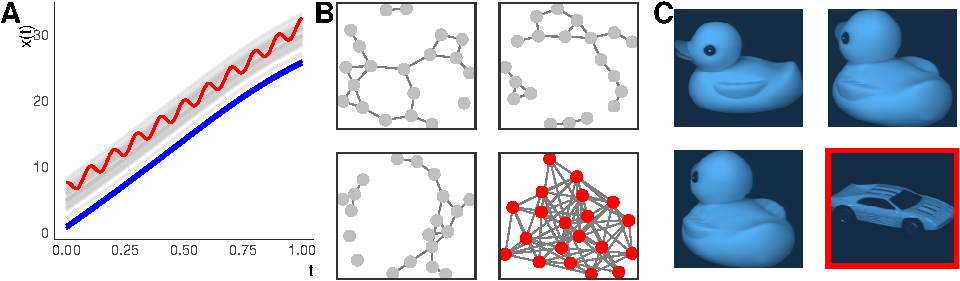
\includegraphics{00_paper_wires_files/figure-latex/outtypes-1.pdf}
\caption{\label{fig:outtypes}\label{fig:outtypes}Example data types. A: Functional inliers (grey) with a structural outlier (red) and distributional outliers (blue). B: Graph data with a structural outlier (lower right graph). C: Image data with a structural outlier (lower right image).}
\end{figure}

In our framework, distributional outliers are defined w.r.t. minimum volume sets (\protect\hyperlink{ref-polonik1997minimum}{Polonik, 1997}) of \(P\) in this parameter space \(\pspace\):

\noindent \textbf{Definition 1:} \emph{Minimum volume set}\\
Given a probability distribution \(P\) over (a subset of) \(\mathbb{R}^d\), a minimum volume set \(\Omega^*_{\alpha}\) is a set that minimizes the quantile function \(V(\alpha) = \inf_{C \in \mathcal{C}}\{\text{Leb}(C): P(C) \geq \alpha\}, 0 < \alpha < 1\)\} for i.i.d. random variables in \(\mathbb{R}^{d}\) with distribution \(P\), \(\mathcal{C}\) a class of measurable subsets in \(\mathbb{R}^{d}\) and Lebesgue measure \(\text{Leb}\).\\
So \(\Omega^*_{\alpha, P}\) is the smallest region containing a probability mass of at least \(\alpha\). We can now define structural outliers and distributional outliers as follows:

\noindent \textbf{Definition 2:} \emph{Structural and distributional outlier}\\
Define \(\mani_{\Theta, \phi}\) as the codomain of \(\phi\) applied to \(\Theta\).\\
Define two such manifolds \(\Man = \mani_{\Than, \phan}\) and \(\Min = \mani_{\Thin, \phin}\) and a data set \(X \subset \Man \cup \Min\).\\
W.l.o.g., let \(r = \frac{\vert \{x_i: x_i \in \Man \land x_i \notin \Min\} \vert}{\vert \{x_i: x_i \in \Min\} \vert} \lll 1\) be the \emph{structural outlier ratio}, i.e.~most observations are assumed to stem from \(\Min\). Then an observation \(x_i \in X\) is

\begin{itemize}
\tightlist
\item
  a \emph{structural outlier} if \(x_i \in \Man\) and \(x_i \notin \Min\) and
\item
  a \emph{distributional outlier} if \(x_i \in \Min\) and \(\theta_i \notin \Omega^*_{\alpha}\), where \(\Omega^*_{\alpha}\) is defined by the density of the distribution generating \(\Than\).
\end{itemize}

Figure \ref{fig:outtypes} shows examples of three data types with structural outliers (in red), and some distributional outliers for the functional data example. Since distributional outliers are structurally similar to inliers, they are hard to detect visually for graph and image data, as doing so requires a lot of ``normal'' data to reference against and we can only display a few example observations here. This is one reason why we mostly use functional data for exposition in the following.

Summarizing the framework's crucial aspects in less technical terms, we assume that the bulk of the observations comes from a single ``common'' process, which generates observations in some subspace \(\Min\), while some data might come from an ``anomalous'' process, which defines structurally distinct observations in a different subspace \(\Man\). This follows standard notions in outlier detection which often assume (at least) two different data-generating processes (\protect\hyperlink{ref-dai2020functional}{Dai et al., 2020}; \protect\hyperlink{ref-zimek2018there}{Zimek \& Filzmoser, 2018}). Note that this does not imply that structural outliers are in any way similar to each other: \(\Pan\) could be very widely dispersed or arise from a mixture or several different distributions and/or \(\Man\) could consist of several unconnected components representing various kinds of structural abnormality. The only crucial aspect is that the process from which \emph{most} of the observations emerge yields structurally similar data.
We consider settings with a structural outlier ratio \(r \in [0, 0.1]\) to be suitable for outlier detection. The proportion of \emph{distributional} outliers on \(\Min\), in contrast, depends only on the \(\alpha\)-level for \(\Omega^*_{\alpha, \Pin}\).
Practically speaking, neither prior knowledge about these manifolds nor specific assumptions about structural differences are necessary in our approach.
The key points are that 1) structural outliers are not on the main data manifold \(\Min\), 2) distributional outliers are at the edges of \(\Min\), and 3) these properties are preserved in the embedding vectors as long as the embedding is based on an appropriate notion of distance in \(\hdspace\).

\section{Experiments}\label{sec:exps}

This section lays out practical implications of the framework through experiments on several different data types, via a comprehensive qualitative and visual analysis of six examples. In addition, we provide quantitative results for three labeled data sets.

\subsection{Methods}\label{sec:exps:meths}

The focus of our experiments is to evaluate a general framework for outlier detection, which is motivated by geometrical considerations. With these experiments, we support the claim that the perspective induced by the framework lets us visualize, detect and analyze outliers in a principled and canonical way. For this demonstration,
we chose Multidimensional Scaling (MDS) (\protect\hyperlink{ref-cox2008multidimensional}{Cox \& Cox, 2008}) as our embedding method and Local Outlier Factors (LOF) (\protect\hyperlink{ref-breunig2000lof}{Breunig et al., 2000}) as our outlier scoring method. Note that the experiments are not intended to
draw conclusions about the superiority of these specific methods and other combinations of methods may be as suitable or even superior for the purpose (see for example results for Isomap in Herrmann \& Scheipl (\protect\hyperlink{ref-herrmann2021geometric}{2021})).\\
However, more sophisticated embedding methods than MDS require tuning over multiple hyperparameters, whereas MDS has only one -- the embedding dimension. Moreover, an advantage of MDS over other embedding methods is that it aims for isometric embeddings, i.e.,
tries to preserve all pairwise distances as closely as possible, which is crucial in particular to reflect structural outlyingness. In fact, Torgerson Multidimensional Scaling (tMDS, i.e., MDS based on \(L_2\) distance) -- that is: a simple linear embedding equivalent to standard PCA scores -- seems to uncover many outlier structures sufficiently well in many data settings despite its simplicity.
For similar reasons, we chose to use LOF as an outlier scoring method. This method also has a single hyperparameter, \(minPts\), the number of nearest neighbors used to define a point's (local) neighborhood, which we denote as \(k\) in the following. Moreover, in contrast to many other outlier scoring methods such one-class support vector machines (\protect\hyperlink{ref-munoz2004one}{Muñoz \& Moguerza, 2004}) which require low-dimensional tabular data as input (i.e.~which can only be applied to complex data types indirectly by using embedding vectors as feature inputs), LOF can also be applied to high-dimensional and non-tabular data directly as it only requires a distance matrix as input. Experiments on functional data have shown that LOF applied directly to a distance matrix of functional data and LOF applied to the corresponding embedding vectors yield consistent results (\protect\hyperlink{ref-herrmann2021geometric}{Herrmann \& Scheipl, 2021}).\\
Note, however, that beyond the ability to apply outlier scoring methods to low-dimensional embedding vectors of high-dimensional and/or non-tabular data, such embeddings provide additional practical value:
In particular, scalar scores or ranks as provided by outlier scoring methods are not able to reflect differences between distributional and structural outliers whereas such differences become accessible and interpretable in visualizations of these embeddings.\\
This also points to a major caveat of the quantitative (in contrast to the qualitative) experiments, in which we use ROC-AUC to evaluate the accuracy of outlier ranks obtained with LOF with respect to the ``outlier'' structure defined by the different classes of labeled data. Setting one class as \(\Min\) and contaminating this ``normal'' class with
observations from other classes, which are assumed to be structurally different and thus form \(\Man\), we obtain data sets \(X \subset \Min \cup \Man\). Although this is a widely used approach (\protect\hyperlink{ref-campos2016evaluation}{Campos et al., 2016}; \protect\hyperlink{ref-goldstein2016comparative}{Goldstein \& Uchida, 2016}; \protect\hyperlink{ref-pang2018learning}{Pang et al., 2018}), such an evaluation only considers outliers as defined by the class labels and poor AUC values may not necessarily imply poor performance if there are observation from the ``normal'' data class which are (distributionally or structurally) more outlying (and thus obtain higher scores) than some of the ``labeled'' outliers, see also Campos et al. (\protect\hyperlink{ref-campos2016evaluation}{2016}). This is why we not merely report potentially problematic quantitative measures (Section \ref{sec:exps:quant}), and instead put more emphasis on qualitative experiments that are much closer to the way we would recommend to use these methods in practical applications.

\subsection{Qualitative assessment}\label{sec:exps:qual}

In this section, we provide extensive qualitative analyses to demonstrate the practical relevance of the framework. First, we demonstrate that the distinction between structural and distributional outliers is preserved in embeddings using two simulated functional data sets. Secondly, using two real world data sets -- a functional and an image data set -- we show that the approach can be applied flexibly to different data structures. Thirdly, we illustrate the general applicability to more general data types based on synthetic graph data and real world curves data. In the following, all LOF results are obtained using \(k = 0.75n\), where \(n\) is the number of observations.

\subsubsection{Demonstrating the framework's practical implications on idealized synthetic data}

Figure \ref{fig:exps-sim} shows two simulated functional data sets (A \& B, left) and their 2\(\vizdim\) PCA/tMDS embeddings (A \& B, right). One can observe that data set A is an example with structural outliers in terms of shape and slope. This is an extended version of an example by Hernández \& Muñoz (\protect\hyperlink{ref-hernandez2106kernel}{2016}) and, following their notation, the two manifolds can be defined as \(\Man = \{x(t) \vert x(t) = b + 0.05t + \cos(20\pi t), b \in \mathbb R\} \cup \{x(t) \vert x(t) = (c - 0.05t) + e_t, c, e_t \in \mathbb R\}\) and \(\Min = \{x(t) \vert x(t) = a + 0.01t + \sin(\pi t^2), a \in \mathbb R\}\) with \(t \in [0, 1]\) and \(a \sim N(\mu = 15, \sigma = 4)\), \(b \sim N(\mu = 5, \sigma = 3)\), \(c \sim N(\mu = 25, \sigma = 3)\), and \(e_t \sim N(\mu = 0, \sigma = 4)\). Note that the structural outliers are not all similar to each other in shape or slope, which is reflected in \(\Min\) being a union of two structurally different manifolds.\\
In contrast, data set B of various (vertically shifted) Beta-distribution densities is an example where distributional outlyingness is defined by phase -- i.e.~horizontal -- variation and structural outlyingness by vertical shifts. The respective manifolds are defined as \(\Man = \{x(t) \vert x(t) = b + B(t, \alpha, \beta), (b, \alpha, \beta)' \in \mathbb R \times \mathbb R^+ \times \mathbb R^+\}\) and \(\Min = \{x(t) \vert x(t) = B(t, \alpha, \beta), (\alpha, \beta)' \in \mathbb R^+ \times \mathbb R^+\}\) with \(t \in [0, 1]\), \(\alpha, \beta \sim U[0.1, 2]\), \(b \sim U[-5, 5]\) and \(B\) the density of the beta distribution. For both, we generate 100 ``normal'' observations from \(\Min\) and 10 structural outliers from \(\Man\), with \(\obsdim = 500\) evaluation points in the first and \(\obsdim = 50\) evaluation points in the latter example.\\
Structural outliers are clearly separated from observations on \(\Min\) in both cases and appear as outlying in the 2\(\vizdim\) embeddings. Moreover, we see that distributional outliers are embedded at the periphery of \(\Min\). Numbers in figures are ascending LOF score ranks of the outliers. Note that \(\Min \subset \Man\) in data set B. Nevertheless, most structurally outlying observations from \(\Man\) are clearly separated in the embedding. Two structural outliers are in or very close to \(\Min \cup \Man\) and thus appear in the main bulk of the data. The LOF scores also reflect this, as one of the distributional outliers is ranked as even more outlying.

\begin{figure}
\centering
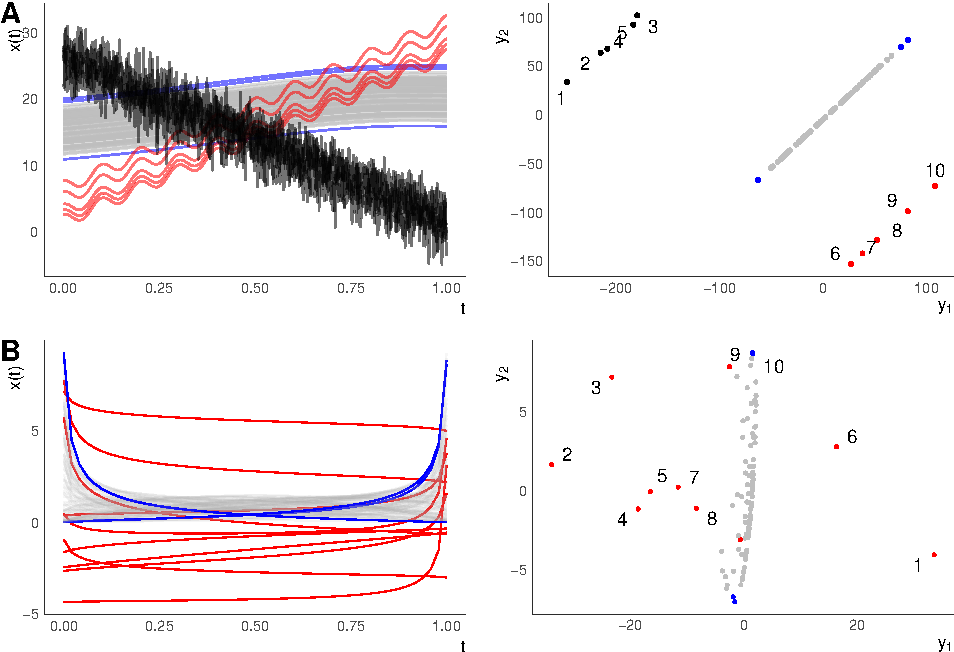
\includegraphics{00_paper_wires_files/figure-latex/fda-simulated-1.pdf}
\caption{\label{fig:fda-simulated}\label{fig:exps-sim} Simulated functional data and their 2\(\vizdim\) embeddings. Numbered labels are ascending LOF score ranks of the outliers (\(k = 0.75n\)).}
\end{figure}

Summarizing, we see that in these simulated situations, practically relevant outlier sub-structure -- deviations in terms of functional shape, slope or in terms of vertical shifts -- are represented accurately by low-dimensional embeddings learned from the observed high-dimensional data. In particular, structural outliers do not need to be similar to each other (Example A) nor do we require that the inlier and outlier manifolds are completely disjoint (Example B) for the approach to work.
Moreover, we see that situations where distributional outliers appear ``more'' outlying than structural outliers are captured as well. Note that this is a crucial aspect. Although this aspect is quantified correctly by an outlier scoring method such as LOF, the two outlier types can be distinguished only if visualizations as provided by embedding methods are considered. Consider that evaluation of unsupervised outlier detection is often performed using a labeled data set, setting observations from one class as inliers and sampling observations from another class as outliers, and then computing binary classification performance measures such as the AUC (\protect\hyperlink{ref-campos2016evaluation}{Campos et al., 2016}; \protect\hyperlink{ref-goldstein2016comparative}{Goldstein \& Uchida, 2016}; \protect\hyperlink{ref-pang2018learning}{Pang et al., 2018}). Different class labels do not guarantee that the classes do not overlap, i.e., that the respective manifolds are disjoint in \(\hdspace\), nor that there are no distributional outliers appearing more outlying than structural outliers. Thus, there may be distributional outliers among the inliers which are scored as more outlying than structural outliers (see data set B) and a purely quantitative assessment is likely to mislead. Being able to create faithful visualizations of such more complex outlier structures for high-dimensional data is a crucial benefit of the proposed approach.

\subsubsection{Demonstrating flexibility on real functional and image data}

Of course, real-world data settings are usually more complicated than our simulated examples. First of all,
real data are much more difficult to assess since the underlying manifolds are usually not directly accessible, so it is impossible to define the exact structure of the data manifolds like in the simulated examples. In addition, some data sets may not contain any clear \textit{structural} outliers, while others may not contain any clear \textit{distributional} outliers, or both. A crucial aspect of the approach is that, although it is based on a highly abstract conceptualization involving unobservables like the parameter space \(\Theta\) and its probability measure \(P\), it is not at all necessary to come up with any such formalization of the data generating process to put the approach into practice and obtain meaningful results, as will be demonstrated in the following.

Consider Figure \ref{fig:fda-image-real}, which shows a real functional data set of 591 ECG measurements (\protect\hyperlink{ref-dau2019ucr}{Dau et al., 2019}; \protect\hyperlink{ref-goldberger2000physiobank}{Goldberger et al., 2000}) with 82 evaluation points per function, i.e.~a \(\obsdim = 82\) dimensional data set (A), and a sample of the COIL20 data (\protect\hyperlink{ref-coil20}{Nane et al., 1996}) (B). Obviously, it is impossible to define the exact structure of the ECG data manifold. However, the visualizations of the functions on the left-hand side suggest that there are no observations with clear structural differences in functional form: none of the curves are clearly shifted away from the bulk of the data, nor are there any curves with isolated peaks or observations with clearly different shapes. In accordance with this observation, there is also no clearly separable structure in the embedding. However, observations which appear in low density regions of the embedding can be regarded as distributional outliers in terms of horizontal shift, i.e., phase variation, like the three observations with the earliest minima colored in blue.
This is also reflected in the scoring of the embeddings, as the observations with the lowest LOF ranks are clear distributional outliers in function space. However, the embedding provides much more complete information in this example than LOF ranks and the functional visualization alone. For example, they also pinpoint a \textit{vertical shift} outlier in the first and last thirds of the domain (green curve, which would be hard to detect based on its functional representation alone). This apparently represents a second ``dimension'' of distributional outlyingness.\\
The COIL20 data (\protect\hyperlink{ref-coil20}{Nane et al., 1996}) consists of 1440 pictures (\(128 \times 128\), gray scale) of 20 different objects. The \(72\) pictures in each class depict one and the same object at different rotation angles with a picture taken at every \(5\)° within \([0\)°\(, 355\)°\(]\).
We use all \(72\) pictures of a rubber duck to represent observations from \(\Min\) and randomly sample \(7\) observations (i.e.~\(r \approx 0.1\)) from the \(72\) pictures of a toy car as structural outliers from \(\Man\). We compute \(L_2\) distances of the vectorized pixel intensities (\(\obsdim = 128^2 = 16384\)).
Figure \ref{fig:fda-image-real} B, left column, shows a sample of \(6\) inlier and \(3\) structural outlier pictures, the right column shows embeddings of all \(79\) images.
Since the inlier data are images of a rotated object, \(\Min\) is the image of a one-dimensional closed and circular parameter space defining the rotation angle (c.f. \protect\hyperlink{ref-ma2011manifold}{Ma \& Fu, 2011}), i.e., other than in the ECG example substantial considerations yield at least some knowledge about the specific structure of the data manifold(s) in this case.

\begin{figure}
\centering
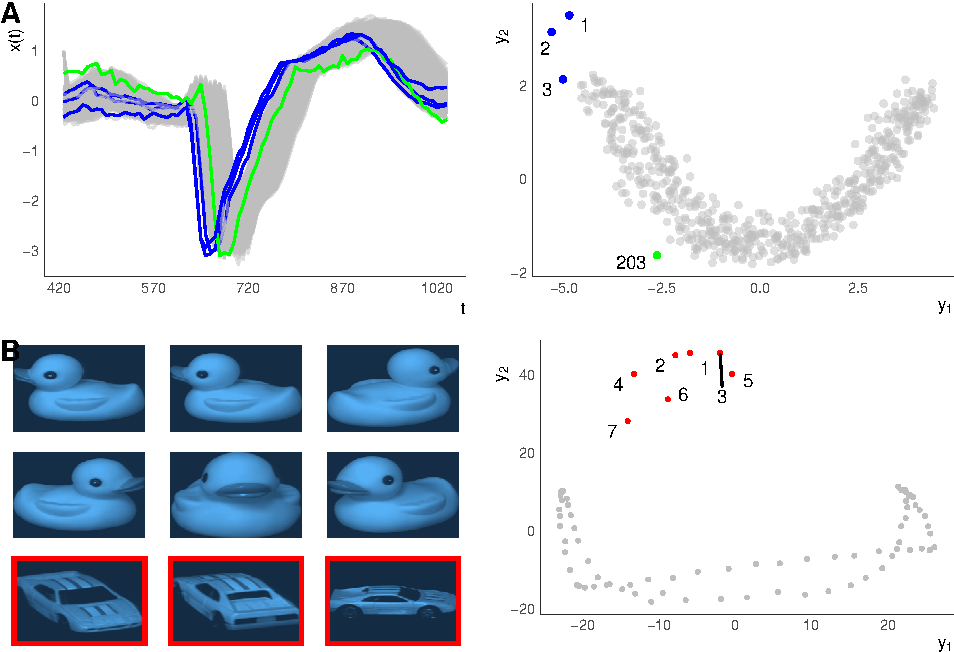
\includegraphics{00_paper_wires_files/figure-latex/fda-image-real-1.pdf}
\caption{\label{fig:fda-image-real}\label{fig:fda-image-real} Real functional and image data and their 2\(\vizdim\) tMDS embeddings. Numbered labels are ascending LOF score ranks of the outliers (\(k = 0.75n\)).}
\end{figure}

The 2\(\vizdim\) embedding reflects the expected structure of our COIL20 subset very well, with clear separation of the \(7\) pictures of the toy car as structural outliers. In addition, the embedding of \(\Min\) indeed yields a closed, but not quite circular loop, as does the embedding of the 7 rotated images from \(\Man\). The corresponding 3D embedding (not shown) reveals that the embeddings of the inliers lie on a rough circle folded over itself.
In summary, in the ECG example there seem to be no clearly separable, structurally different outliers which could be detected with tMDS, but only distributional outliers, whereas in the COIL data there are clearly separate structural outliers, but no distributionally outlying observations. These two examples with very different intrinsic structures (single connected manifold with distributional outliers versus disconnected manifolds without clear distributional outliers) illustrate that it is not necessary to have explicit prior knowledge about the data generating process or its outlier characteristics for the approach to work and that it is able to handle different data manifold structures flexibly and successfully.

\subsubsection{Demonstrating generalizability on graph and curve data}

Note that the COIL example illustrates that the framework also works in image data and that a fairly simplistic approach of computing \(L_2\) distances between vectorized pixel intensities yields very reasonable results in this example.
The framework is, however, not at all restricted to these two data types nor to such a simple distance metric. Recall that the approach can be applied to any data type whatsoever as long as a suitable distance metric is available. Beyond 1\(\vizdim\) functional and image data, the framework can also be extended to more general and complex data types, for example graphs or 2\(\vizdim\) curves as depicted in Figure \ref{fig:further-qual-exp}. We use more specialized distance measures to show that good results can also be obtained on such data.\\
We simulate two structurally different classes of Erd\H{o}s-Rényi graphs with 20 vertices (see Fig. \ref{fig:further-qual-exp} A). This structural difference results from different edge probabilities \(p_v\) that two given vertices of the graph are connected, setting \(p_{v} = 0.1\) for \(\Min\) and \(p_{v} = 0.4\) for \(\Man\). We randomly sample \(100\) observations from \(\Min\) and \(10\) from \(\Man\), i.e.~\(r = 0.1\), and obtain a pairwise distance matrix by computing the Frobenius distances between the graph Laplacians.

\begin{figure}
\centering
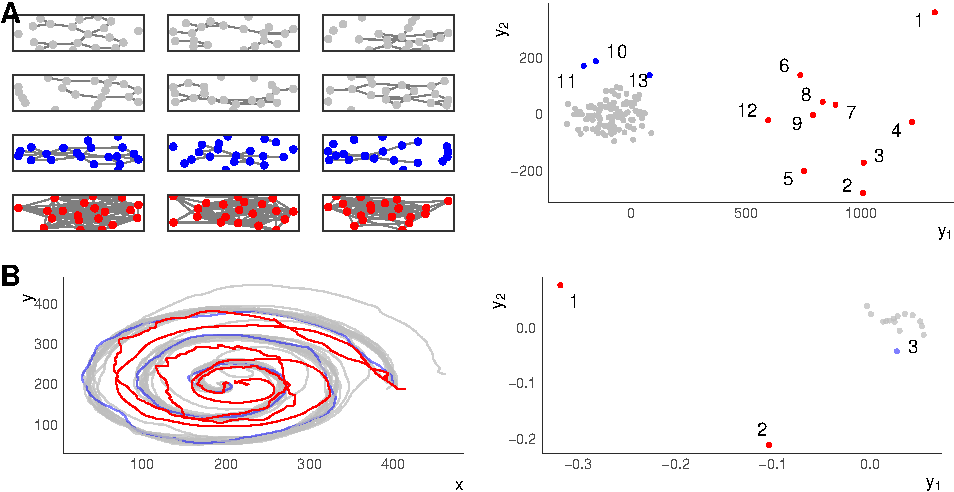
\includegraphics{00_paper_wires_files/figure-latex/further-qual-exp-1.pdf}
\caption{\label{fig:further-qual-exp}\label{fig:further-qual-exp} Curve and graph data as further examples to demonstrate the flexibility and general applicability of the approach, and their 2\(\vizdim\) MDS embeddings based on Frobenius (graphs) and Elastic shape distances (curves). Numbered labels are ascending LOF score ranks of the outliers (\(k = 0.75n\)).}
\end{figure}

The curves data (Fig. \ref{fig:further-qual-exp} B) consists of spiral curve drawings from an Archimedes spiral-drawing test that is used to diagnose patients with Parkinson's disease (\protect\hyperlink{ref-alty2017use}{Alty et al., 2017}; \protect\hyperlink{ref-steyer2021elastic}{Steyer et al., 2021}). Taking data from the dynamic version of the test (\protect\hyperlink{ref-isenkul2014improved}{Isenkul et al., 2014}), we use 15 curves drawn by healthy controls not suffering from Parkinson's disease and two curves drawn by Parkinson patients to represent potential structural outliers, where each curve is evaluated on 200 points. Previous investigations have shown that an elastic shape distance is better suited than \(L_2\) distances to discriminate between the two groups (\protect\hyperlink{ref-steyer2021elastic}{Steyer et al., 2021}).\\
So, in contrast to the previous examples, we use more specialized distance measures to capture the relevant structures in these settings. This illustrates that the approach is not only flexible with respect to the actual structure present in a given data set as demonstrated in the previous section, but that it is also very generally applicable to a variety of data types. The approach can be used for any kind of data simply by defining an appropriate (data-specific) distance measure.
In both the embeddings of the graphs as well as the embeddings of the curves, structurally different observations (in red) are clearly separated from the observations on \(\Min\). This is also reflected by their LOF scores. Moreover, in both settings there are observations from \(\Min\) (in blue) which appear in peripheral, sparser regions of the ``normal'' data and thus can be considered distributional outliers.
Note that it is not always immediately obvious on the level of the original data why observations appear distributionally outlying. For example, in the graph data, note that other than in previous examples (e.g.~Fig. \ref{fig:exps-sim} A) comparing them to a few inliers does not reveal striking difference at first (in contrast to the structural outliers!): Figure \ref{fig:further-qual-exp} A, left column, shows six inlier graphs in the 1st and 2nd row, the three distributional outlier graphs in the 3rd row, and three structural outlier graphs in the 4th row.\\
Nevertheless, the embedding vectors and their LOF ranks indicate that the distributionally outlying observations have obtained some specific characteristics setting them apart from most inlying observations. For example, further analysis reveals that the graph with LOF rank 11 contains the node with maximum connectedness of all nodes in all inlier graphs. Its degree is 8 (i.e., it is directly connected to 8 other nodes), while the average of the maximum degree in the graphs on \(\Min\) is just 4.39. In contrast, the graph with LOF rank 13 contains 8 isolated nodes of degree 0, while the average number of nodes with with degree 0 is only 2.47 on \(\Min\). The respective values of the graph with LOF rank 10 are above the upper quartile for both of these metrics, with 4 unconnected nodes and a maximally connected node with degree 6.

\hypertarget{quantitative-assessment}{%
\subsection{\texorpdfstring{Quantitative assessment \label{sec:exps:quant}}{Quantitative assessment }}\label{quantitative-assessment}}

In order to provide less subjective experimental results, we assess the approach quantitatively, using labeled data with at least two classes. For each data set, we consider four outlier ratios \(r \in \{0.01, 0.025, 0.5, 0.1\}\). Setting one class as \(\Min\), with \(n_{in} = \vert \Min \vert\), and contaminating this ``normal'' class with \(n_{out} = r \cdot n_{in}\) ``structural'' outliers from other classes, which form \(\Man\), we obtain data sets \(X \subset \Min \cup \Man\) with \(n = n_{in} + n_{out}\). For each setting, we repeat the contamination process 50 times, sampling outliers at random from \(\Man\). Based on outlier ranks computed with LOF, we use ROC-AUC as a performance measure and report the mean AUCs over the 50 replications for each combination of settings. Note that we only use the labels of the ``structural'' outliers for computing this performance measure, not for the unsupervised learning of the embeddings themselves.
For all data sets considered in this section, plots of typical embeddings for \(r = 0.05\) can be found in Figure \ref{fig:app} in the appendix.
We consider three additional functional data sets for this experiment: \textit{dodgers} (\protect\hyperlink{ref-dau2019ucr}{Dau et al., 2019}), a set of times series of daily traffic close to Dodgers Stadium, with days on weekends forming \(\Man\) and weekdays forming \(\Min\); \textit{phoneme} (\protect\hyperlink{ref-febrero2012fdausc}{Febrero-Bande \& Oviedo de la Fuente, 2012}), discretized log-periodograms of five different phonemes, with phoneme ``dcl'' forming \(\Man\) and phonemes ``sh'', ``iy'', ``aa'', and ``ao'' forming \(\Min\); \textit{starlight} (\protect\hyperlink{ref-dau2019ucr}{Dau et al., 2019}; \protect\hyperlink{ref-rebbapragada2009finding}{Rebbapragada et al., 2009}), phase-aligned light curves of Eclipsing Binary, Cepheid, and RR Lyrae stars, the first forming \(\Man\) and the latter two forming \(\Min\). All results are based on simple, linear tMDS/PCA embeddings with the LOF algorithm applied to the resulting 2\(\vizdim\) embedding vectors.\\
The results show that outlier detection does not need to be specifically challenging in nominally high dimensional data. In each of the data sets, which have very different number of observations and number of dimensions, high ROC-AUC \(\geq 0.95\) can be achieved for all considered outlier ratios \(r\). This indicates that most of the observations from \(\Man\) indeed appear to be outlying in the embedding space and thus obtain high LOF scores. Furthermore, as in the qualitative analysis, a global setting of \(k = 0.75n\) seems to be a reasonable default for the LOF algorithm. Only for \(r = 0.01, 0.025\) in the starlight data,
we see a large improvement (AUC \(= 1.00\)) with \(k = 0.1n\). For small \(r < 0.1\), in all other settings the achieved ROC-AUC is very robust against changes in this tuning parameter.

\begin{table}
\scriptsize
\caption{\label{tab:real-quant}Mean ROC-AUC values over 50 replications based on the ranks as assigned by LOF. Each data set consists of $n$ observations, $n_{in}$ from $\Min$ and $n_{out} = n_{in} \cdot r$ from $\Man$. $\Man$ and $\Min$ are defined by classes of the original labeled data sets. $D$ is the dimensionality of a data set (i.e, evaluations per function for functional data) and $k$ the number of nearest neighbors used in the LOF algorithm.}
\centering
\resizebox{\textwidth}{!}{\begin{tabular}{@{}lcccccrccccrcccc@{}} \toprule
\textbf{} & & \multicolumn{4}{c}{dodgers} & & \multicolumn{4}{c}{phoneme} & & \multicolumn{4}{c}{starlight} \\
 & & \multicolumn{4}{c}{$n_{in} = 97$, $\obsdim = 289$} & & \multicolumn{4}{c}{$n_{in} = 400$, $\obsdim = 150$} & & \multicolumn{4}{c}{$n_{in} = 6656$, $\obsdim = 1025$} \\
\cmidrule{3-6} \cmidrule{8-11} \cmidrule{13-16}
 & $k$       & $0.01n$ & $0.1n$ & $0.75n$ & $0.9n$ & & $0.01n$ & $0.1n$ & $0.75n$ & $0.9n$ & & $0.01n$ & $0.1n$ & $0.75n$ & $0.9n$ \\  \midrule
$r: 1.0\%$ & & 0.78 & 0.98 & 0.96 & 0.96 & & 0.78 & 1.00 & 0.99 & 0.99 & & 0.96 & 1.00 & 0.69 & 0.78 \\
$r: 2.5\%$ & & 0.62 & 0.97 & 0.96 & 0.96 & & 0.54 & 1.00 & 0.99 & 0.99 & & 0.55 & 1.00 & 0.88 & 0.88 \\
$r: 5.0\%$ & & 0.59 & 0.97 & 0.96 & 0.96 & & 0.56 & 0.99 & 0.99 & 0.99 & & 0.53 & 1.00 & 0.92 & 0.92 \\
$r: 10\%$  & & 0.54 & 0.84 & 0.97 & 0.96 & & 0.57 & 0.75 & 0.99 & 0.99 & & 0.56 & 0.98 & 0.95 & 0.87\\
\bottomrule
\end{tabular}}
\end{table}

\hypertarget{sec:discussion}{%
\section{Discussion}\label{sec:discussion}}

\hypertarget{sec:discussion:implications}{%
\subsection{Summary}\label{sec:discussion:implications}}

We propose a geometrically motivated framework for outlier detection, which exploits the metric structure of a (possibly high-dimensional) data set and provides a mathematically precise distinction between \emph{distributional} outliers and \emph{structural} outliers. Experiments show that the outlier structure of high-dimensional and non-tabular data can be detected, visualized and quantified using established manifold learning methods and standard outlier scoring. The decisive advantage of our framework from a theoretical perspective is that the resulting embeddings make subtle but important properties of outlier structure explicit and -- even more importantly -- that these properties are made accessible based on visualizations of the embeddings. From a more practical perspective, our proposal requires no prior knowledge nor any specific assumptions about the actual data structure in order to work, an important aspect since data generating processes are usually inaccessible. This is highly relevant in practice, in particular since a well established, computationally cheap combination of widely used and fairly simple methods like (t)MDS and LOF proved to be a strong baseline that yields fairly reliable results without the need for tuning hyperparameters. In addition, the proposed framework has several more general conceptual implications for outlier detection which will be summarized in the following.

\hypertarget{sec:disc:implications}{%
\subsection{Implications}\label{sec:disc:implications}}

\textbf{Outlier taxonomy} We propose a clear taxonomy to distinguish between frequently interchangeably used terms \emph{anomalies} and \emph{outliers} in a canonical way: we regard \emph{anomalies} as observations from a different data generating process than the majority of the data (i.e.~as observations that are on \(\Man\) but not on \(\Min\)), which can be more precisely identified as \emph{structural} outliers. Recall that Zimek and Filzmoser (\protect\hyperlink{ref-zimek2018there}{2018, p. 10}) refer to such observations as ``real'' outliers that need to be distinguished from ``observations which are in the extremes of the model distribution''. On the other hand, regarding \emph{outliers} as observations from low density regions of the underlying ``normal'' data manifold \(\Min\), they can be more precisely identified as \emph{distributional} outliers.
Based on our reading of the literature, this distinction is usually not made explicit. Since there is rarely a practical reason to assume that a given data set contains only \textit{distributional} or only \textit{structural} outliers, some of the confusion surrounding the topic (\protect\hyperlink{ref-goldstein2016comparative}{Goldstein \& Uchida, 2016}; \protect\hyperlink{ref-unwin2019multivariate}{Unwin, 2019}; \protect\hyperlink{ref-zimek2018there}{Zimek \& Filzmoser, 2018}) might be due to the fact that such conceptual differences have not been made sufficiently clear.
As outlined, the concept of structural difference is very general. For example, structural differences in functional data may appear as shape anomalies in data mainly characterized by vertical shift variation (see Fig. \ref{fig:outtypes} A) or as vertical shift anomalies in data dominated by shape variation, as phase anomalies in data with magnitude variation or magnitude anomalies in data with phase variation, etc.\\
In real unlabeled data, there may not always be a clear distinction between somewhat structurally anomalous observations with ``off-manifold'' embeddings and merely distributionally outlying observations with embeddings on the periphery of the data manifold, as in the ECG data in Figure \ref{fig:fda-image-real} A. Nevertheless, the theoretical distinction between these two kinds of outliers adds conceptual clarity even if the practical application of the categories may not be straightforward.\\
\textbf{Curse of dimensionality} As outlined in section \ref{sec:prelims:scope}, outlier detection is often reported to suffer from the curse of dimensionality. For example, Goldstein \& Uchida (\protect\hyperlink{ref-goldstein2016comparative}{2016}) show that most outlier detection methods under consideration break down or perform poorly in a data set with 400 dimensions and conclude that unsupervised outlier detection is not possible in such high dimensions. Some {[}Aggarwal (\protect\hyperlink{ref-aggarwal2017outlier}{2017}); e.g.{]} attribute this to the fundamental problem that distance functions can lose their discriminating power in high dimensions (\protect\hyperlink{ref-beyer1999nearest}{Beyer et al., 1999}), which is linked to the the concentration of measure effect (\protect\hyperlink{ref-pestov2000geometry}{Pestov, 2000}). However, this effect occurs only under fairly specific conditions (\protect\hyperlink{ref-zimek2012survey}{Zimek et al., 2012}), which means that outlier detection does not have to be affected by the curse of dimensionality: In addition to the effects of dependency structures and signal-to-noise ratios (\protect\hyperlink{ref-zimek2012survey}{Zimek et al., 2012}), the necessary conditions for concentration of measure are not fulfilled if the intrinsic dimensionality of the data is smaller than the actually observed dimensionality, or if the data is distributed in clusters that are relatively well separable (\protect\hyperlink{ref-beyer1999nearest}{Beyer et al., 1999}). Exactly these two characteristics are reflected in our framework in the form of (1) the manifold assumption, which implies low-ish intrinsic dimensionality, and (2) the assumption that structural outliers come from different manifolds than the rest of the data, i.e., from different ``clusters'' in \(\hdspace\). This has two important consequences: First of all, the geometric perspective our framework is based on makes these important aspects for outlier detection in high-dimensional data explicit, while a purely probabilistic perspective obscures them. Secondly, it mitigates many of the problems associated with high-dimensional outlier detection: any outlier detection method that performs well in low dimensions becomes -- in principle -- applicable in nominally high-dimensional and/or complex non-tabular data when applied to suitable low dimensional embedding coordinates.
In addition, our results show that outlier sub-structure, specifically the differences between distributional and structural outliers, can be detected and visualized with manifold methods. This opens new possibilities for descriptive and exploratory analyses:\\
\textbf{Visualizability of outlier characteristics} If the embeddings provided by manifold methods are restricted to two or three dimensions, they also provide easily accessible visualizations of the data. In fact, manifold learning is often used in applications specifically to find two- or three-dimensional visualizations reflecting the essential intrinsic structure of the high-dimensional data as faithfully as possible. Consequently, structural and distributional outliers, which are rather glaring data characteristics if the manifolds are well separable, can often be separated clearly even in two or three dimensional representations as long as the embedding is (approximately) isometric with respect to a suitable dissimilarity measure. This is specifically important for complex non-tabular or high-dimensional data types such images or graphs where at most a few observations can be visualized and perceived simultaneously. In the same vein, substructures and notions of data depth are reflected in the embeddings, making the approach also useful as an exploration tool for settings with unclear structure.\\
\textbf{Generalizability} Since the central building block of the proposed framework is to capture the metric structure of data sets using distance measures, the framework is very general and applicable to any data types for which distance metrics are available. In Section \ref{sec:exps:qual}, we illustrated this generalizability using high-dimensional as well as non-tabular data; in particular we applied it to functional, curve, graph, and image data. This also makes the framework very flexible as one can make use of non-standard and customized dissimilarity measures to emphasize the relevant structural differences in specific situations based on domain knowledge: Representing image data as vectors of pixel intensities, we computed distances between those vectors, for example. Dissimilarities between different graphs were captured, for example, by constructing their graph Laplacians and computing Frobenius distances between them, and we used a specific elastic depth distance for the spiral curve data as suggested by earlier results in Steyer et al. (\protect\hyperlink{ref-steyer2021elastic}{2021}).

\hypertarget{sec:discussion:limitations}{%
\subsection{Limitations and outlook}\label{sec:discussion:limitations}}

Inliers, i.e.~observations on \(\Min\), may show large ``within class'' variation and/or may be spread over several disconnected clusters in some situations. For example, object images on \(\Min\), which are structurally similar in terms of the depicted objects' shape, may vary in rotation, scale, or location, and may have different color or texture. In functional data, observations on \(\Min\) may show phase and amplitude variation and form clusters due to different shapes. In such settings, \(\Min\) can yield complex substructure and highly dispersed observations and it may be hard to distinguish whether separable structures observed in embeddings are due to groups of homogeneous structural outliers or due to multimodality in \(\Min\) in which some modes are sparsely sampled. Moreover, in such cases, the dispersion of \(\Min\) accounts for large parts of the data's variability and two or three dimensional MDS embeddings may not be sufficient to also faithfully represent structural outliers, since MDS embedding vectors are sorted decreasingly by explained ``variance''. However, this does not mean that structural outliers are not necessarily separable. Instead, they appear as outliers in higher embedding dimensions, requiring higher order embeddings to reflect the outlier structure. To some extent, scatterplot matrices visualizing the embedding dimensions of such higher order embeddings in a pairwise manner can be used for visualization in such situations (\protect\hyperlink{ref-herrmann2021geometric}{Herrmann \& Scheipl, 2021}). In other settings, however, techniques from multi-view learning such as ``distance-learning from multiple views'' may likely yield better results, because different structures (e.g.~structure induced by color vs structure induced by texture) should be ``treated separately as they are \emph{semantically} different'' (\protect\hyperlink{ref-zimek2015blind}{Zimek \& Vreeken, 2015, p. 128}). Note, however, that suitable inductive biases can also be brought to bear in our framework fairly easily. If substantial considerations suggest that specific structural aspects are important, specifying dissimilarity metrics focused on these aspects allows to emphasize the relevant differences. For example, if isolated outliers in functional data (i.e.~functions which yield outlying behavior only over small parts of the domain such as isolated peaks) are of most interest, higher order \(L_p\) metrics such as \(L_{10}\) will be much more sensitive to such structural differences than general \(L_2\) distances. If phase variation should be ignored, the unnormalized \(L_1\)-Wasserstein or the Dynamic Time Warping (DTW) distance can be used. Such problem-specific distance measures can reduce the number of MDS embedding dimensions necessary for faithful embeddings of structural outliers (\protect\hyperlink{ref-herrmann2021geometric}{Herrmann \& Scheipl, 2021}). In future work, we will investigate these aspects and possible extensions w.r.t. to multi-view learning approaches. Moreover, we will elaborate more on the specifics of other data types, in particular, image data.

\hypertarget{sec:conclusion}{%
\section{Conclusion}\label{sec:conclusion}}

In conclusion, our illustration suggests that the proposed geometric conceptualization, which distinguishes \emph{distributional} and \emph{structural} outlier on a general level, provides a more precise terminology and shows that outlier detection in high-dimensional and complex non-tabular data does need to be specifically challenging per se. Convincing results could be achieved in a wide range of settings and data types by a combination of the simple methods MDS for dimension reduction and visualization and LOF for outlier scoring. We hope that the proposed framework contributes to a better understanding of unsupervised outlier detection and provides some guidance to practitioners as well as methodological researchers in this regard.

\section*{Funding}

This work has been funded by the German Federal Ministry of Education and Research (BMBF) under Grant No.~01IS18036A. The authors of this work take full responsibility for its content.

\section*{Acknowledgment}

The authors thank Almond Stöcker for his helpful advice regarding the spiral curve data.

\section*{Conflict of interest}

The authors have declared no conflicts of interest for this article.

\section*{Data availability statement}

The data and code to reproduce the findings of this study are openly available on GitHub at:
\url{https://github.com/HerrMo/geo-outlier-framework}

\section*{References}

\hypertarget{refs}{}
\begin{CSLReferences}{1}{0}
\leavevmode\vadjust pre{\hypertarget{ref-aggarwal2017outlier}{}}%
Aggarwal, C. C. (2017). \emph{Outlier analysis} (2nd ed.). Springer. \url{https://doi.org/10.1007/978-3-319-47578-3}

\leavevmode\vadjust pre{\hypertarget{ref-aggarwal2001outlier}{}}%
Aggarwal, C. C., \& Yu, P. S. (2001). Outlier detection for high dimensional data. \emph{SIGMOD Rec.}, \emph{30}(2), 37--46. \url{https://doi.org/10.1145/376284.375668}

\leavevmode\vadjust pre{\hypertarget{ref-ali2019timecluster}{}}%
Ali, M., Jones, M. W., Xie, X., \& Williams, M. (2019). Time{C}luster: Dimension reduction applied to temporal data for visual analytics. \emph{The Visual Computer}, \emph{35}(6), 1013--1026. \url{https://doi.org/10.1007/s00371-019-01673-y}

\leavevmode\vadjust pre{\hypertarget{ref-alty2017use}{}}%
Alty, J., Cosgrove, J., Thorpe, D., \& Kempster, P. (2017). How to use pen and paper tasks to aid tremor diagnosis in the clinic. \emph{Practical Neurology}, \emph{17}(6), 456--463. \url{https://doi.org/10.1136/practneurol-2017-001719}

\leavevmode\vadjust pre{\hypertarget{ref-azcorra2018unsupervised}{}}%
Azcorra, A., Chiroque, L. F., Cuevas, R., Anta, A. F., Laniado, H., Lillo, R. E., Romo, J., \& Sguera, C. (2018). Unsupervised scalable statistical method for identifying influential users in online social networks. \emph{Scientific Reports}, \emph{8}(1), 1--7. \url{https://doi.org/10.1038/s41598-018-24874-2}

\leavevmode\vadjust pre{\hypertarget{ref-belkin2003laplacian}{}}%
Belkin, M., \& Niyogi, P. (2003). Laplacian eigenmaps for dimensionality reduction and data representation. \emph{Neural Computation}, \emph{15}(6), 1373--1396. \url{https://doi.org/10.1162/089976603321780317}

\leavevmode\vadjust pre{\hypertarget{ref-beyer1999nearest}{}}%
Beyer, K., Goldstein, J., Ramakrishnan, R., \& Shaft, U. (1999). When is {``nearest neighbor''} meaningful? In C. Beeri \& P. Buneman (Eds.), \emph{Database theory --- ICDT'99} (pp. 217--235). Springer Berlin Heidelberg. \url{https://doi.org/10.1007/3-540-49257-7_15}

\leavevmode\vadjust pre{\hypertarget{ref-breunig2000lof}{}}%
Breunig, M. M., Kriegel, H.-P., Ng, R. T., \& Sander, J. (2000). {LOF}: Identifying density-based local outliers. \emph{SIGMOD Rec.}, \emph{29}(2), 93--104. \url{https://doi.org/10.1145/335191.335388}

\leavevmode\vadjust pre{\hypertarget{ref-campos2016evaluation}{}}%
Campos, G. O., Zimek, A., Sander, J., Campello, R. J., Micenková, B., Schubert, E., Assent, I., \& Houle, M. E. (2016). On the evaluation of unsupervised outlier detection: Measures, datasets, and an empirical study. \emph{Data Mining and Knowledge Discovery}, \emph{30}(4), 891--927. \url{https://doi.org/10.1007/s10618-015-0444-8}

\leavevmode\vadjust pre{\hypertarget{ref-clemenccon2013scoring}{}}%
Clémençon, S., \& Jakubowicz, J. (2013). Scoring anomalies: A {M}-estimation formulation. In C. M. Carvalho \& P. Ravikumar (Eds.), \emph{Proceedings of the sixteenth international conference on artificial intelligence and statistics} (Vol. 31, pp. 659--667). PMLR. \url{https://proceedings.mlr.press/v31/clemencon13a.html}

\leavevmode\vadjust pre{\hypertarget{ref-coifman2006diffusion}{}}%
Coifman, R. R., \& Lafon, S. (2006). Diffusion maps. \emph{Applied and Computational Harmonic Analysis}, \emph{21}(1), 5--30. \url{https://doi.org/10.1016/j.acha.2006.04.006}

\leavevmode\vadjust pre{\hypertarget{ref-cox2008multidimensional}{}}%
Cox, M. A. A., \& Cox, T. F. (2008). Multidimensional scaling. In \emph{Handbook of data visualization} (pp. 315--347). Springer Berlin Heidelberg. \url{https://doi.org/10.1007/978-3-540-33037-0_14}

\leavevmode\vadjust pre{\hypertarget{ref-dai2020functional}{}}%
Dai, W., Mrkvička, T., Sun, Y., \& Genton, M. G. (2020). Functional outlier detection and taxonomy by sequential transformations. \emph{Computational Statistics \& Data Analysis}, \emph{149}, 106960. \url{https://doi.org/10.1016/j.csda.2020.106960}

\leavevmode\vadjust pre{\hypertarget{ref-dau2019ucr}{}}%
Dau, H. A., Bagnall, A., Kamgar, K., Yeh, C.-C. M., Zhu, Y., Gharghabi, S., Ratanamahatana, C. A., \& Keogh, E. (2019). The {UCR} time series archive. \emph{IEEE/CAA Journal of Automatica Sinica}, \emph{6}(6), 1293--1305. \url{https://doi.org/10.1109/JAS.2019.1911747}

\leavevmode\vadjust pre{\hypertarget{ref-febrero2012fdausc}{}}%
Febrero-Bande, M., \& Oviedo de la Fuente, M. (2012). Statistical computing in functional data analysis: The {R} package {fda.usc}. \emph{Journal of Statistical Software}, \emph{51}(4), 1--28. \url{https://doi.org/10.18637/jss.v051.i04}

\leavevmode\vadjust pre{\hypertarget{ref-fritsch2012detecting}{}}%
Fritsch, V., Varoquaux, G., Thyreau, B., Poline, J.-B., \& Thirion, B. (2012). Detecting outliers in high-dimensional neuroimaging datasets with robust covariance estimators. \emph{Medical Image Analysis}, \emph{16}(7), 1359--1370. \url{https://doi.org/10.1016/j.media.2012.05.002}

\leavevmode\vadjust pre{\hypertarget{ref-goldberger2000physiobank}{}}%
Goldberger, A. L., Amaral, L. A., Glass, L., Hausdorff, J. M., Ivanov, P. C., Mark, R. G., Mietus, J. E., Moody, G. B., Peng, C.-K., \& Stanley, H. E. (2000). Physio{B}ank, {P}hysio{T}oolkit, and {P}hysio{N}et: Components of a new research resource for complex physiologic signals. \emph{Circulation}, \emph{101}(23), e215--e220. \url{https://doi.org/10.1161/01.CIR.101.23.e215}

\leavevmode\vadjust pre{\hypertarget{ref-goldstein2016comparative}{}}%
Goldstein, M., \& Uchida, S. (2016). A comparative evaluation of unsupervised anomaly detection algorithms for multivariate data. \emph{PloS One}, \emph{11}(4), e0152173. \url{https://doi.org/10.1371/journal.pone.0152173}

\leavevmode\vadjust pre{\hypertarget{ref-hernandez2106kernel}{}}%
Hernández, N., \& Muñoz, A. (2016). Kernel {D}epth {M}easures for {F}unctional {D}ata with {A}pplication to {O}utlier {D}etection. In A. E. P. Villa, P. Masulli, \& A. J. Pons Rivero (Eds.), \emph{Artificial neural networks and machine learning -- {ICANN} 2016} (pp. 235--242). Springer, Cham. \url{https://doi.org/10.1007/978-3-319-44781-0_28}

\leavevmode\vadjust pre{\hypertarget{ref-herrmann2021geometric}{}}%
Herrmann, M., \& Scheipl, F. (2021). A geometric perspective on functional outlier detection. \emph{Stats}, \emph{4}(4), 971--1011. \url{https://doi.org/10.3390/stats4040057}

\leavevmode\vadjust pre{\hypertarget{ref-isenkul2014improved}{}}%
Isenkul, M., Sakar, B., Kursun, O., et al. (2014). Improved spiral test using digitized graphics tablet for monitoring parkinson's disease. \emph{The 2nd International Conference on e-Health and Telemedicine (ICEHTM-2014)}, \emph{5}, 171--175.

\leavevmode\vadjust pre{\hypertarget{ref-kamalov2020outlier}{}}%
Kamalov, F., \& Leung, H. H. (2020). Outlier detection in high dimensional data. \emph{Journal of Information \& Knowledge Management}, \emph{19}(01), 2040013. \url{https://doi.org/10.1142/S0219649220400134}

\leavevmode\vadjust pre{\hypertarget{ref-kandanaarachchi2020dimension}{}}%
Kandanaarachchi, S., \& Hyndman, R. J. (2020). Dimension reduction for outlier detection using {DOBIN}. \emph{Journal of Computational and Graphical Statistics}, 1--16. \url{https://doi.org/10.1080/10618600.2020.1807353}

\leavevmode\vadjust pre{\hypertarget{ref-large2018}{}}%
Large, J., Kemsley, E. K., Wellner, N., Goodall, I., \& Bagnall, A. (2018). Detecting forged alcohol non-invasively through vibrational spectroscopy and machine learning. In D. Phung, V. S. Tseng, G. I. Webb, B. Ho, M. Ganji, \& L. Rashidi (Eds.), \emph{Advances in knowledge discovery and data mining} (pp. 298--309). Springer International Publishing. \url{https://doi.org/10.1007/978-3-319-93034-3_24}

\leavevmode\vadjust pre{\hypertarget{ref-lee2007nonlinear}{}}%
Lee, J. A., \& Verleysen, M. (2007). \emph{Nonlinear {Dimensionality} {Reduction}} (1st ed.). Springer Science \& Business Media. \url{https://doi.org/10.1007/978-0-387-39351-3}

\leavevmode\vadjust pre{\hypertarget{ref-loperfido2020kurtosis}{}}%
Loperfido, N. (2020). Kurtosis-based projection pursuit for outlier detection in financial time series. \emph{The European Journal of Finance}, \emph{26}(2-3), 142--164. \url{https://doi.org/10.1080/1351847X.2019.1647864}

\leavevmode\vadjust pre{\hypertarget{ref-ma2011manifold}{}}%
Ma, Y., \& Fu, Y. (Eds.). (2011). \emph{Manifold learning theory and applications} (1st ed.). CRC press. \url{https://doi.org/doi.org/10.1201/b11431}

\leavevmode\vadjust pre{\hypertarget{ref-maaten2008visualizing}{}}%
Maaten, L. van der, \& Hinton, G. (2008). Visualizing data using t-{SNE}. \emph{Journal of Machine Learning Research}, \emph{9}(86), 2579--2605. \url{http://jmlr.org/papers/v9/vandermaaten08a.html}

\leavevmode\vadjust pre{\hypertarget{ref-marques2020internal}{}}%
Marques, H. O., Campello, R. J., Sander, J., \& Zimek, A. (2020). Internal evaluation of unsupervised outlier detection. \emph{ACM Transactions on Knowledge Discovery from Data (TKDD)}, \emph{14}(4), 1--42. \url{https://doi.org/10.1145/3394053}

\leavevmode\vadjust pre{\hypertarget{ref-mcinnes2018umap}{}}%
McInnes, L., Healy, J., \& Melville, J. (2018). \emph{{UMAP}: Uniform manifold approximation and projection for dimension reduction}. arXiv. \url{https://doi.org/10.48550/ARXIV.1802.03426}

\leavevmode\vadjust pre{\hypertarget{ref-munoz2004one}{}}%
Muñoz, A., \& Moguerza, J. M. (2004). One-class support vector machines and density estimation: The precise relation. In A. Sanfeliu, J. F. Martínez Trinidad, \& J. A. Carrasco Ochoa (Eds.), \emph{Progress in pattern recognition, image analysis and applications} (pp. 216--223). Springer Berlin Heidelberg. \url{https://doi.org/10.1007/978-3-540-30463-0_27}

\leavevmode\vadjust pre{\hypertarget{ref-coil20}{}}%
Nane, S., Nayar, S., \& Murase, H. (1996). Columbia object image library: COIL-20. \emph{Dept. Comp. Sci., Columbia University, New York, Tech. Rep}.

\leavevmode\vadjust pre{\hypertarget{ref-navarro2021high}{}}%
Navarro-Esteban, P., \& Cuesta-Albertos, J. A. (2021). High-dimensional outlier detection using random projections. \emph{TEST}, \emph{30}(4), 908--934. \url{https://doi.org/10.1007/s11749-020-00750-y}

\leavevmode\vadjust pre{\hypertarget{ref-pang2018learning}{}}%
Pang, G., Cao, L., Chen, L., \& Liu, H. (2018). Learning representations of ultrahigh-dimensional data for random distance-based outlier detection. \emph{Proceedings of the 24th ACM SIGKDD International Conference on Knowledge Discovery \& Data Mining}, 2041--2050. \url{https://doi.org/10.1145/3219819.3220042}

\leavevmode\vadjust pre{\hypertarget{ref-pestov2000geometry}{}}%
Pestov, V. (2000). On the geometry of similarity search: Dimensionality curse and concentration of measure. \emph{Information Processing Letters}, \emph{73}(1-2), 47--51. \url{https://doi.org/10.1016/S0020-0190(99)00156-8}

\leavevmode\vadjust pre{\hypertarget{ref-polonik1997minimum}{}}%
Polonik, W. (1997). Minimum volume sets and generalized quantile processes. \emph{Stochastic Processes and Their Applications}, \emph{69}(1), 1--24. \url{https://doi.org/10.1016/S0304-4149(97)00028-8}

\leavevmode\vadjust pre{\hypertarget{ref-ramsay2005functional}{}}%
Ramsay, J. O., \& Silverman, B. W. (2005). \emph{Functional data analysis} (2nd ed). Springer. \url{https://doi.org/10.1007/b98888}

\leavevmode\vadjust pre{\hypertarget{ref-rebbapragada2009finding}{}}%
Rebbapragada, U., Protopapas, P., Brodley, C. E., \& Alcock, C. (2009). Finding anomalous periodic time series. \emph{Machine Learning}, \emph{74}(3), 281--313. \url{https://doi.org/10.1007/s10994-008-5093-3}

\leavevmode\vadjust pre{\hypertarget{ref-ren2017projection}{}}%
Ren, H., Chen, N., \& Zou, C. (2017). Projection-based outlier detection in functional data. \emph{Biometrika}, \emph{104}(2), 411--423. \url{https://doi.org/10.1093/biomet/asx012}

\leavevmode\vadjust pre{\hypertarget{ref-ro2015outlier}{}}%
Ro, K., Zou, C., Wang, Z., \& Yin, G. (2015). Outlier detection for high-dimensional data. \emph{Biometrika}, \emph{102}(3), 589--599. \url{https://doi.org/10.1093/biomet/asv021}

\leavevmode\vadjust pre{\hypertarget{ref-rousseeuw2005robust}{}}%
Rousseeuw, P. J., \& Leroy, A. M. (2005). \emph{Robust regression and outlier detection}. John Wiley \& Sons. \url{https://doi.org/10.1002/0471725382}

\leavevmode\vadjust pre{\hypertarget{ref-roweis2000nonlinear}{}}%
Roweis, S. T., \& Saul, L. K. (2000). Nonlinear dimensionality reduction by locally linear embedding. \emph{Science}, \emph{290}(5500), 2323--2326. \url{https://doi.org/10.1126/science.290.5500.2323}

\leavevmode\vadjust pre{\hypertarget{ref-scott2006learning}{}}%
Scott, C. D., \& Nowak, R. D. (2006). Learning minimum volume sets. \emph{The Journal of Machine Learning Research}, \emph{7}(24), 665--704. \url{http://jmlr.org/papers/v7/scott06a.html}

\leavevmode\vadjust pre{\hypertarget{ref-steyer2021elastic}{}}%
Steyer, L., Stöcker, A., \& Greven, S. (2021). \emph{Elastic analysis of irregularly or sparsely sampled curves}. arXiv. \url{https://doi.org/10.48550/ARXIV.2104.11039}

\leavevmode\vadjust pre{\hypertarget{ref-tenenbaum2000global}{}}%
Tenenbaum, J. B., Silva, V. de, \& Langford, J. C. (2000). A {Global} {Geometric} {Framework} for {Nonlinear} {Dimensionality} {Reduction}. \emph{Science}, \emph{290}(5500), 2319--2323. \url{https://doi.org/10.1126/science.290.5500.2319}

\leavevmode\vadjust pre{\hypertarget{ref-thudumu2020comprehensive}{}}%
Thudumu, S., Branch, P., Jin, J., \& Singh, J. J. (2020). A comprehensive survey of anomaly detection techniques for high dimensional big data. \emph{Journal of Big Data}, \emph{7}(1), 1--30. \url{https://doi.org/10.1186/s40537-020-00320-x}

\leavevmode\vadjust pre{\hypertarget{ref-toivola2010novelty}{}}%
Toivola, J., Prada, M. A., \& Hollmén, J. (2010). Novelty detection in projected spaces for structural health monitoring. In P. R. Cohen, N. M. Adams, \& M. R. Berthold (Eds.), \emph{Advances in intelligent data analysis IX} (pp. 208--219). Springer Berlin Heidelberg. \url{https://doi.org/10.1007/978-3-642-13062-5_20}

\leavevmode\vadjust pre{\hypertarget{ref-unwin2019multivariate}{}}%
Unwin, A. (2019). Multivariate outliers and the {O}3 plot. \emph{Journal of Computational and Graphical Statistics}, \emph{28}(3), 635--643. \url{https://doi.org/10.1080/10618600.2019.1575226}

\leavevmode\vadjust pre{\hypertarget{ref-xie2017geometric}{}}%
Xie, W., Kurtek, S., Bharath, K., \& Sun, Y. (2017). A {G}eometric {A}pproach to {V}isualization of {V}ariability in {F}unctional data. \emph{Journal of the American Statistical Association}, \emph{112}(519), 979--993. \url{https://doi.org/10.1080/01621459.2016.1256813}

\leavevmode\vadjust pre{\hypertarget{ref-xu2018comparison}{}}%
Xu, X., Liu, H., Li, L., \& Yao, M. (2018). A comparison of outlier detection techniques for high-dimensional data. \emph{International Journal of Computational Intelligence Systems}, \emph{11}(1), 652--662. \url{https://doi.org/10.2991/ijcis.11.1.50}

\leavevmode\vadjust pre{\hypertarget{ref-zhang2006anomaly}{}}%
Zhang, J., \& Zulkernine, M. (2006). Anomaly based network intrusion detection with unsupervised outlier detection. \emph{2006 IEEE International Conference on Communications}, \emph{5}, 2388--2393. \url{https://doi.org/10.1109/ICC.2006.255127}

\leavevmode\vadjust pre{\hypertarget{ref-zimek2018there}{}}%
Zimek, A., \& Filzmoser, P. (2018). There and back again: Outlier detection between statistical reasoning and data mining algorithms. \emph{Wiley Interdisciplinary Reviews: Data Mining and Knowledge Discovery}, \emph{8}(6), e1280. \url{https://doi.org/10.1002/widm.1280}

\leavevmode\vadjust pre{\hypertarget{ref-zimek2012survey}{}}%
Zimek, A., Schubert, E., \& Kriegel, H.-P. (2012). A survey on unsupervised outlier detection in high-dimensional numerical data. \emph{Statistical Analysis and Data Mining: The ASA Data Science Journal}, \emph{5}(5), 363--387. \url{https://doi.org/10.1002/sam.11161}

\leavevmode\vadjust pre{\hypertarget{ref-zimek2015blind}{}}%
Zimek, A., \& Vreeken, J. (2015). The blind men and the elephant: On meeting the problem of multiple truths in data from clustering and pattern mining perspectives. \emph{Machine Learning}, \emph{98}(1), 121--155. \url{https://doi.org/10.1007/s10994-013-5334-y}

\end{CSLReferences}

\newpage

\appendix

\hypertarget{sec:app}{%
\section{Example visualizations of the data used in the quantitative experiments}\label{sec:app}}

\begin{figure}
\centering
\includegraphics{00_paper_wires_files/figure-latex/app-1.pdf}
\caption{\label{fig:app}\label{fig:app} Plots to Table 1: Functional data and tMDS embeddings. Inlier class in grey, outlier class in red. \(r = 0.05\)}
\end{figure}

\end{document}
